\documentclass[11pt]{book}

\usepackage[utf8]{inputenc}
\usepackage[spanish]{babel}
\usepackage{hyperref}
\usepackage{graphicx}
\usepackage{subcaption}
\usepackage{txfonts}
%\usepackage{csquotes}
%\usepackage{babelbib}
%\usepackage{authblk}
%\usepackage{makeidx}

%\makeatletter
\newcommand{\chapterauthor}[1]{%
  {\parindent0pt\vspace*{-25pt}%
  \linespread{1.1}\large\scshape#1%
  \par\nobreak\vspace*{35pt}}
  \@afterheading%
}
%\makeatother

\newcommand{\mysection}[2]
  {{\renewcommand{\sectionmark}[1]{}
    \section{#1}}\sectionmark{#2}}
    
\title{Manual de la asignatura Ingeniería de Software de Fuentes Abiertas/Libre - versión 2022}
\author{Ricardo Medel y colaboradores}

\begin{document}
\date{}
\maketitle

\tableofcontents
%\listoffigures
%\listoftables

\chapter*{Prefacio}
\addcontentsline{toc}{chapter}{Prefacio}

Este texto es producto de un ejercicio de trabajo colaborativo utilizando herramientas digitales que son usadas regularmente en comunidades de software libre\footnote{Herramientas utilizadas: el sistema de control de versiones Git, la plataforma de repositorios GitHub y el procesador de textos \LaTeX.}, realizado entre los años 2016 y 2018. Si bien su ambicioso título es \emph{Manual de la asignatura Ingeniería de Software de Fuentes Abiertas/Libre}, más bien debe considerarse como una serie de apuntes sobre los diferentes temas abordados en esta asignatura electiva (de quinto nivel) de la carrera de Ingeniería en Sistemas de Infomación de la Facultad Regional Córdoba de la Universidad Tecnológica Nacional.

Estos apuntes, entonces, no deben tomarse como el texto definitivo de la asignatura, ya que ninguno de los capítulos cubre todos los aspectos de cada tema ni profundiza en ellos. Más bien, se recomienda utilizarlo como una base para comenzar una exploración más profunda de cada tema, a partir de las referencias y enlaces provistos.

Como todo trabajo colaborativo, este texto es la suma de los aportes de cada autor/a y la interacción entre autores/as, por lo que se puede notar cierta heterogeneidad en los estilos de escritura y los enfoques con los que se aborda cada tema. Hemos hecho ciertos intentos de homogeneización del estilo del texto, pero aún queda trabajo por hacer en ese sentido.

Durante los años en que se escribió y modificó este texto, muchas han sido las personas que hicieron sus aportes, no todas dejaron su registro\footnote{Si considerás que sos autor/a y no se te incluyó en esta lista, por favor, enviame un email a \texttt{rmedel@frc.utn.edu.ar} indicando que participaste en la creación de este manual.}, por lo que esta lista puede estar incompleta: 
Pablo Bajo,
Luciano Bartoszensky,
Federico Benito,
Agustín Borello,
Braian Chincho,
Nahuel Ignacio Cuello,
Alexis Donato,
Manolo Fernández, 
Facundo Ferrero,
Juan Filardo,
Máximo Fiora, 
Mayco Garelli,   
Marcos López,
Carlos Luna,
Paolo Mattio,
Ricardo Medel,
Fernando Meichtri,
Diego Moreno Moreyra, 
Jeremías Niño,
Federico Prado,
Fernanda Pucheta, 
Julieta Ríos,
Mauricio Sánchez,
Lucas Martín Segurado,
Fabricio Simoncelli,
Milena Vilardo,
Gonzalo Ulla,
Fernando Zamora.

A todas ellas y todos ellos, va el agradecimiento de la cátedra, por su aporte a este texto que nos permite tener un punto de partida en común para poder desarrollar cada uno de los temas que abordamos en esta asignatura única en su tipo, al menos por ahora, en todo el país.
 
Si las lectoras o los lectores encuentran errores o quieren aportar mejoras, son libres de hacerlo por su propia iniciativa, ya que este documento tiene licencia libre y su código fuente está accesible en un repositorio público\footnote{\url{}}.

\parbox{2in}{\vspace{2in}}
\hfill
\parbox{2in}%
{Ricardo Medel\\%
Córdoba, 8 de marzo de 2022\\%
\mbox{}} 

Este trabajo está licenciado bajo la Creative Commons Attribution-ShareAlike 4.0 International License (\url{http://creativecommons.org/licenses/by-sa/4.0/}).



\chapter{Introducción al software libre}
\label{capIntro}
%\chapterauthor{Fernandez Manolo, Fiora Máximo, Garelli Mayco, Luna Carlos, Meichtri Fernando, Sanchez Mauricio}


En este capítulo hacemos una revisión ligera de los principales hitos históricos del software libre, para lo cual necesitamos presentar algunos conceptos técnicos y legales, tales como la definición de software libre, las licencias de software o los sistemas operativos. Aquí algunos de estos conceptos son abordados someramente, pero volveremos sobre ellos con más detalles en los siguientes capítulos.

\section{Historia del software libre}

Si bien la historia del software libre es relativamente corta, sus principales eventos, sus protagonistas y, especialmente, sus efectos en la informática tal como la conocemos son abundantes, interesantes y muy ricos desde el punto de vista histórico. Gran cantidad de artículos, libros y hasta películas\footnote{\emph{Revolution OS} es una película de 85 minutos sobre la historia del software libre desde sus comienzos hasta 2001. \url{http://revolution-os.com/}} sobre este tema han sido realizados. En esta sección nos proponemos realizar apenas una aproximación a su historia, proveyendo abundante bibliografía para que el o la lectora interesada pueda profundizar a su gusto.

Desde que en los años `50 la creciente miniaturización de los componentes electrónicos permitió la comercialización de computadoras y hasta comienzos de los años `70, aproximadamente, la mayoría de las compañías que producían computadoras digitales o periféricos tenían el hábito de dejar a disposición de los usuarios el código fuente (archivos legibles) de su software. Si algún usuario o grupo de usuarios realizaba mejoras a ese software, estas mejoras eran compartidas en las comunidades de usuarios de dichas computadoras e incluso las empresas adoptaban estas mejoras. Esto se debía principalmente a que las comunidades de usuarios eran pequeñas, ya que los costos tanto de las computadoras como de la infraestructura y mano de obra requerida para operar eran prohibitivos y por lo tanto se vendían apenas unas decenas de cada modelo, y también a que el software funcionaba solamente en el hardware para el que había sido escrito.

A comienzos de los `70 los avances de la década anterior en el desarrollo de sistemas operativos y compiladores permitieron el nacimiento de la industria del software como un fenómeno separado del hardware. De esta forma, el código fuente pasó a tener un valor comercial que antes no tenía y comenzaron las tensiones entre quienes comercializaban software y quienes lo consideraban una herramienta que debería estar al alcance de todos para su mayor desarrollo. Dos anécdotas, separadas casi por una década, marcaron esa tensión y una de ellas generaría un importante cambio en la cultura del desarrollo de software.

En febrero de 1976 Bill Gates, apenas meses después de fundar la empresa Microsoft, publicó una ``Carta abierta a los aficionados''\footnote{``Open Letter to Hobbyists'', por su título original en inglés~\cite{gates76}.}, en la que consideraba que lo que los aficionados al desarrollo de software llamaban \emph{compartir} era en realidad, y en sus palabras, \emph{robar} y eso impedía el desarrollo profesional de software. 

A principios de la década del `80 Richard Stallman, mientras trabajaba en el Laboratorio de Inteligencia Artificial del Instituto Tecnológico de Massachusetts (MIT), quiso hacer unas modificaciones al software de una impresora Xerox y se encontró con que el código fuente no estaba disponible y aquellos investigadores que sí tenían acceso a dicho código habían firmado acuerdos de no revelarlo\footnote{NDA, Non-Disclosure Agreement, en inglés.}. Este fue uno de los incidentes\footnote{Otro posible evento fue el desacuerdo entre Stallman y Symbolics, Inc. sobre el acceso a las actualizaciones que Symbolics había realizado a su máquina Lisp, la cual estaba basada en código de libre acceso realizado por el MIT.} que llevaron a Richard Stallman a dedicar su vida a la creación del movimiento del software libre~\cite{williams02}, comenzando entre 1983 y 1985 con el proyecto GNU\footnote{\url{https://www.gnu.org/}} para el desarrollo de un sistema operativo similar al entonces famoso Unix\footnote{GNU's Not Unix, es un acrónimo recursivo que significa ``GNU No es Unix''}, la publicación de ``El manifiesto de GNU''\footnote{\url{https://www.gnu.org/gnu/manifesto.es.html}} y la creación de la Fundación Software Libre\footnote{FSF, Free Software Foundation en inglés. \url{https://www.fsf.org/}}.

En la sección siguiente daremos una definición más precisa del Software Libre, pero por ahora será suficiente indicar que es aquel software que permite a los y las usuarias utilizarlo, modificarlo y distribuirlo sin restricciones.

Desde medidados de los años `80 el software libre y el movimiento sociopolítico que lo rodea no han parado de crecer. Sin embargo, a comienzos de los `90 el proyecto GNU había desarrollado muchas de las herramientas informáticas requeridas para un sistema operativo (editores de texto, compiladores, etc.) pero no tenía un componente clave: el núcleo (o \emph{kernel}, en inglés). Fue en 1991 que, paralelamente al proyecto GNU y aprovechando la posibilidad de realizar desarrollo distribuido gracias a la creciente difusión de la Internet, un estudiante finlandés, Linus Torvalds, comenzó el desarrollo de un núcleo libre, con características similares a Unix, el cual se llamaría Linux. Esta pieza vino a completar todos los componentes requeridos para tener un sistema operativo libre, conocido como GNU/Linux.

Aproximadamente para la misma época, en 1994, se lanzaba la versión totalmente libre del sistema operativo BSD\footnote{BSD por \emph{Berkeley Software Distribution}.}, también derivado de Unix. Este sistema y sus diferentes versiones han tenido cierto éxito, pero no puede compararse con la amplia difusión de las versiones de GNU/Linux, llamadas \emph{distribuciones} o \emph{distros}.

Hacia fines de la década de los `90 el movimiento de software libre había crecido, especialmente impulsado por la Internet, la cual permite a los y las desarrolladoras de software trabajar en forma distribuida desde prácticamente cualquier lugar del mundo y, asimismo, distribuir el software sin los costos asociados a los canales de comercialización tradicionales. Sin embargo, poco impacto se había logrado en el mundo de los negocios y las grandes empresas, y varias personas mostraron su disconformidad con las fuertes posiciones políticas de Richard Stallman. Fue así que en 1998, Bruce Perens, Eric S. Raymond y  Jon ``Maddog'' Hall, entre otras personas, crearon la Iniciativa de Fuentes Abiertas (OSI, por sus siglas en inglés\footnote{\emph{Open Source Initiative}, \url{https://opensource.org/}}). Su motivación es menos política y más pragmática, haciendo hincapié en las ventajas técnicas y económicas del software que pone el código fuente a disposición de todos los y las usuarias.

El mismo año de creación de la OSI, el navegador de internet Netscape, que unos años antes había sido el de mayor penetración de mercado (hasta 90\%), liberó su código como respuesta a la agresiva campaña de Microsoft para imponer su navegador Internet Explorer. La creación de la OSI y la liberación del código de Netscape tuvieron un significativo impacto comercial y durante el resto de la década, y hasta la explosión de la así llamada \emph{burbuja puntocom}, fueron muchas las compañías basadas en software libre o software de fuentes abiertas que comenzaron a cotizar en bolsa con valuaciones millonarias.

En los últimos años, la difusión del software libre ha sido muy importante, excepto en las computadoras personales (ya sea de escritorio o portátiles) donde el sistema operativo mayoritario sigue siendo alguna versión de MS Windows. Donde el software libre es más fuerte es en los servidores que prestan servicios a través de Internet. Allí, el \textit{stack} de software está generalmente constituido por diferentes distribuciones de GNU/Linux y servidores web libres, tales como Nginx o Apache. Así mismo, desde el año 2017 todas las supercomputadoras en el top500, el ranking de las computadoras más veloces del mundo, creado en 1995, corren bajo alguna versión de Linux.

% algo sobre las startups con web apps basadas en software libre.
En la actualidad, el software libre permite la creación rápida de \textit{start ups} tecnológicas, ya que reduce los costos iniciales de desarrollo de las herramientas de software necesarias (evitando tanto el autodesarrollo como el pago de licencias por software privativo durante las etapas iniciales del negocio) y permite la adaptación a los requisitos particulares del nuevo emprendimiento~\cite{kamau16, singh21, gerasimenko16, wiggers21}. 

Completamos esta suerte de historia general del software libre y de fuentes abiertas con dos hitos anecdóticos que marcan sendos momentos en que el éxito en la difusión del software libre fue remarcado (en formas totalmente diferentes) por expresiones públicas de representantes de la empresa que supo encarnar todo lo opuesto al software libre, Microsoft. 

\begin{itemize}
\item En junio de 2001 el por entonces gerente general de Microsoft, Steve Ballmer, dijo en un reportaje que ``Linux es un cancer que contagia, en el sentido de propiedad intelectual, a todo lo que toca.''\footnote{La cita original es ``Linux is a cancer that attaches itself in an intellectual property sense to everything it touches.'' La entrevista original ya no está disponible en el sitio del Chicago Sun-Times, pero un análisis (en inglés) de la noticia aún puede leerse en The Register\cite{theregister01}.}

\item En una charla durante un evento en octubre de 2014 el por entonces nuevo gerente general de Microsoft, Satya Nadella, presentó la nueva posición de la empresa ante el software libre, resumiéndola con una filmina que decía ``Microsoft $\varheartsuit$ Linux''.\footnote{Grabación de la charla de Nadella: \url{https://youtu.be/54hHr8ye2kE}}

\end{itemize}


%\section{Conceptos del Software Libre y de Fuentes Abiertas}
%\sectionmark{Conceptos}

\mysection{Conceptos del software libre y de fuentes abiertas}{Conceptos}

Comenzamos formalizando la definición de {\it Software Libre} tal como la estableció Richard Stallman como parte del proyecto GNU: aquel software cuyos términos de uso (su licencia) le aseguran a los y las usuarias las siguiente cuatro libertades esenciales.

\begin{enumerate}
\setcounter{enumi}{-1}
\item La libertad de utilizar el software con cualquier propósito.
\item La libertad de estudiar el programa y modificarlo para adaptarlo a las propias necesidades.
\item La libertad de distribuir copias del programa.
\item La libertad de distribuir copias de las versiones modificadas del programa.
\end{enumerate}

Cabe destacar que las libertades 1 y 3 requieren de acceso al \emph{código fuente}, es decir, los archivos conteniendo el software en un formato legible por un ser humano (y por un compilador o intérprete). Por lo que se puede considerar que una característica fundamental del Software Libre es que sea de \emph{Fuentes Abiertas}\footnote{\emph{Open Source}, en inglés.}. 

Como dijimos previamente, la creación en 1998 de la \emph{Open Source Initiative} tenía como objetivo hacer más amigable al software libre con el ámbito de los negocios. Además de cambiar el confuso (en inglés) nombre de Software Libre al más neutro Fuentes Abiertas, se estableció una definición alternativa, aunque conceptualmente similar. Para la OSI, un software es de Fuentes Abiertas si cumple con los siguientes 10 criterios.

\begin{enumerate}
\item {\bf Redistribución libre}: La licencia no restringirá el derecho de vender o regalar el software como parte de un paquete de software. No se podrá requerir el pago de tasas por las ventas.

\item {\bf Código fuente}: El programa debe incluir el código fuente y debe permitir la distribución de dicho código y de su forma compilada. Si el producto no se distribuye con el código fuente, debe haber una forma clara de obtenerlo por no más que un costo razonable de reproducción, preferentemente descargándolo de la Internet en forma gratuita. El código fuente debe ser la forma preferida en que un/a programador/a modifique el programa. Código ofuscado deliberadamente no es aceptable. Formas intermedias, como el resultado de un preprocesador o un traductor no son permitidas.

\item {\bf Trabajos derivados}: La licencia debe permitir modificaciones y trabajos derivados, y permitir que sean distribudos bajo los mismos términos que la licencia del software original.

\item {\bf Integridad del código fuente del/la autor/a}: La licencia puede restringir la distribución de modificaciones del código fuente solo si permite la distribución de "parches" con el código fuente que modifiquen el programa al momento de construcción (\emph{build}) La licencia debe permitir explícitamente la distribución del software construido a partir del código modificado. La licencia puede requerir que los trabajos derivados tengan un nombre o número de versión diferentes del software original.

\item {\bf No discriminación contra personas o grupos}: La licencia no debe discriminar a ninguna persona o grupo de personas.

\item {\bf No discriminación contra actividades}: La licencia no debe restringir a nadie de hacer uso del programa en una actividad específica. 

\item {\bf Distribución de licencia}: Los derechos vinculados a un programa deben aplicarse a todas las partes a las que les es redistribuido sin la necesidad de licencias adicionales para dichas partes.

\item {\bf La licencia no debe ser específica para un producto}: Los derechos vinculados a un programa no deben depender de que tal programa sea parte de una distribución particular de software. Si el programa es extraído de dicha distribución y utilizado o distribuido respetando los términos de su licencia, todas las partes a quienes el programa es redistribuido deben tener los mismos derechos que han sido otorgados en conjunto con la distribución original.

\item {\bf La licencia no debe restringir otro software}: La licencia no debe establecer restricciones sobre otro software que sea distribuido junto con el software sobre el cual se aplica dicha licencia. 

\item {\bf La licencia debe ser tecnológicamente neutral}: Ninguna parte de la licencia debe basarse en una tecnología o estilo de interfaz específicos.

\end{enumerate}

Aunque las definiciones en principio lucen muy diferentes, realmente no establecen un concepto diferente para el software libre o de fuentes abiertas. La principal diferencia entre la Free Software Foundation, promotora del término y definición del software libre, y la Open Source Inititative, promotora del software de fuentes abiertas, está en sus motivaciones fundamentales.

La FSF argumenta que el software es conocimiento y debe poderse difundir sin trabas. Ocultar el conocimiento es una actitud antisocial y moralmente reprensible. Además, la posibilidad de estudiar y modificar programas es una forma de libertad de expresión.

Por su parte la OSI tiene una motivación más pragmática, argumentando que el software de fuentes abiertas tiene ventajas técnicas y económicas que solo se logran compartiendo el código fuente.

En ese aspecto, existe alguna confusión respecto a que el software libre es igual a software gratuito. En principio, como se mencionó arriba, la primera confusión viene del término \emph{free software}, ya que \emph{free} en inglés significa tanto ``libre'' como ``gratuito''\footnote{Nótese que en español a veces también se utilizan ambos términos en forma similar, por ejemplo, cuando se indica que en una fiesta hay ``barra libre''.}. Es por eso que, jocosamente, Richard Stallman aclara que el software es \emph{free as in Freedom, not as in free beer}\footnote{El software es libre como en libertad, no como en cervezas gratis.}.

Por otro lado, es cierto que en general se puede acceder al software libre en forma gratuita, ya que al requerirse el acceso al código fuente y su posibilidad de distribuirlo (por las libertades 1 y 3), el costo del software, o mejor dicho de su código binario, tiende a cero: la empresa o comunidad desarrolladora lo puede vender pero sus primeros clientes lo pueden distribuir en forma legal (ya sea por menor costo o gratuitamente), por lo que los clientes siguientes no tendrán la necesidad de adquirirlo al precio establecido por sus desarrolladores. Como veremos más adelante, esto no impide que se puedan hacer negocios basados en software libre. Simplemente, no tiene sentido cobrar por utilizarlo, tal cual es el modelo de negocios tradicional en la industria del software.

Por completitud mencionaremos el \emph{freeware} o \emph{shareware} que, aunque ya no sean tan comunes esos términos, definen a software que es gratuito o que se comparte gratuitamente. en algunos casos con funciones reducidas (se de pagar para acceder a más funciones) y otros con la posibilidad de realizar pagos voluntarios a sus autores. La principal diferencia con software libre es que este tipo de software puede no ofrecer algunas de las libertades requeridas para ser definido como tal. Generalmente no se permite ni el acceso al código fuente, ni su modificación, ni la distribución de dichas modificaciones.

%
%\section{Leyes que favorecieron al software libre}
%
%{\bf Ley aprobada en la región de Piamonte Italia}
%\\
%\\
%En 2010 el Consejo Regional de Piamonte, una región nordoccidental de Italia, que limita con Suiza al norte y con Francia al oeste, aprobaba una Ley, que establecía que se favorecerá a los programas pertenecientes a la categoría del software libre y a los programas en los que el código es inspeccionable por el licenciatario.

%La elección fue acogida con entusiasmo por los partidarios del Software Libre y una gran parte de la sociedad civil, mientras que la Presidencia del Consejo de Ministros impugnaba esta norma, pidiendo al Tribunal Constitucional que la declarara ilegal. Pero el Tribunal a cargo del juicio dictaminó que la preferencia por el software Libre es legal y respeta el principio de la libre competencia.

%Como veredicto determinaron que, preferir Software Libre no infringe la libertad de competencia, ya que la libertad del software es una característica jurídica de carácter general y no una característica tecnológica ligada a un producto o marca específica. Esta sentencia expuso la inconsistencia de los argumentos que, durante mucho tiempo, se han opuesto a la adopción de normas que favorezcan la utilización de Software Libre argumentando que están en conflicto con el principio de "neutralidad tecnológica".


%\section{El Software Libre en Latinoamérica y el Caribe}
%\sectionmark{El software libre en Latinoamérica} 

\mysection{El software libre en Latinoamérica y el Caribe}{El software libre en LAC}

Latinoamérica y el Caribe son regiones consumidoras de tecnología, ya sea importada de otras partes del mundo o producida localmente por sucursales de compañías extranjeras. A partir de los procesos de privatización y desregularización de las telecomunicaciones llevados adelante en los años '80 y '90, los servicios también están dominados por gigantes globales. La mayoría del software propietario líder en el mercado ha sido traducido a español y portugués en busca de un mercado creciente.

El software libre, si bien no con la fuerza que tiene en países centrales, también tiene su cuota de desarrollo en esta región. Mencionaremos algunos hitos y organizaciones que así lo muestran. No incluimos en este somero listado las diferentes organizaciones y eventos que surgieron a lo largo del tiempo y luego desaparecieron o se discontinuaron, ya que eso queda para un relevamiento histórico más completo.

El programador brasileño Marcelo Tosatti desde noviembre de 2001, cuando tenía solo 18 años, se convirtió en el mantenedor y co-mantenedor de ciertas versiones del kernel Linux. 

El software de escritorio Gnome fue iniciado por los programadores mexicanos Miguel de Icaza y Federico Mena, forma parte oficial del proyecto GNU y es uno de los escritorios más utilizados por distribuciones GNU/Linux.

El evento FLISoL (Festival Latinoamericano de Instalación de Software Libre)\footnote{\url{https://flisol.info/}} se realiza desde el año 2005 simultáneamente en diferentes ciudades de países latinoamericanos. Comenzó como un encuentro presencial para instalar distribuciones de sistemas operativos en computadoras que los usuarios acercaran al evento, pero actualmente es un evento que incluye otras actividades, como charlas, talleres, presentaciones y ferias.

El Proyecto Software Libre de Brasil (\emph{Software Livre Brasil} en portugués) es una red de personas e instituciones creada a principios de los años 2000 con el objetivo de promover el uso y desarrollo de software libre como una alternativa de libertad económica, tecnológica y de expresión en ese país\footnote{\url{http://softwarelivre.org/portal/quem-somos}}. En su momento de mayor auge pudo promover el desarrollo y uso de software libre en los gobiernos de varios estados de Brasil y del gobierno federal, así como la organización del Foro Internacional de Software Libre, que durante 18 años se llevó a cabo en Porto Alegre.


%{\bf Caso Android. ¿ Android es Software Libre?}
%\\
%\\
%Android. Android es un \emph{software de código abierto} que se distribuye bajo la licencia Apache V2.
%\\
%La licencia Apache V2 da permiso para:
%\\
%Utilizar el software para cualquier propósito, distribuirlo, modificarlo y distribuir las modificaciones
%no tiene copyleft por lo que las versiones modificadas no tienen que ser distribuidas como software libre.
%Compatible con GPL3 pero no con las anteriores.
%Incluye provisiones de protección respecto a patente.
%\\
%Android es un software de código abierto con  acceso al código fuente del mismo, pero terceras partes, como por ejemplo fabricantes, pueden modificarlo o añadir código y este no tiene porqué ser liberado. 
%\\
%Leer mas en: https://www.androidsis.com/android-es-software-libre-estamos-en-lo-cierto/

%\section{Conclusion}
%	
%Gracias a la cultura de compartir el conocimiento (El software) la industria al dia de hoy se vio afectada favorablemente, derivando en importantes desarrollos como lo fueron Unix, BSD, TCP/IP, etc.
%Cuando las empresas en su afán de consolidar su posición en el mercado, entendieron que el software era un activo valioso decidieron que esta no debía ser compartido tan a la ligera, dando lugar a las NDA y al software privativo.
%\\
%En este movimiento se han cometido muchos abusos, hasta patentar y registrar cosas triviales que permiten a las empresas demandar a otras por un Doble Click, ¡literalmente! (Registro de Microsoft).
%\\
%Ya hace tiempo, las empresas también entendieron  que no solo el software es un activo importantes, sino, aún más valioso son los datos generados por estos. Dando lugar a una proliferación de software gratuito o de código abierto con el objetivo de obtener datos de lo más variado y estos ser usados con fines estratégicos y/o comerciales.
%\\
%Cuando no tenemos el código fuente no es posible saber como este esta hecho, tampoco como este funciona, ya que no es transparente. 
%Solo si sabemos como funciona el software podemos hablar de transparencia y solo cuando tenemos acceso a modificar el funcionamiento del software estamos habilitados a dejar ser simples consumidores.
%\\
%La distinción crucial del software es justamente ésta: el acceso a poder entender cómo funciona y poder modificarlo. 
%\\
%Como usuarios debemos entender cómo estas empresas actúan, aceptando o rechazando sus prácticas.
%\\
%Otra observación sobre las grandes corporaciones y su software privativo es el empoderamiento a través de estrategias destinadas a copar el mercado con sus producto y estableciendolos como protocolos defactos.
%El usuario domestico solo es una arista menor, siendo su principal interes las empresas que deberan adaptarse a las tecnologias dispuesta en el mercado, que mediane la renovación constante de licencias y actulizaciones generan la depencia buscada.
%\\
%Si todos usan una misma tecnologia, esta se vuelve el standar, provocando un efecto contagio.
%\\
%\emph{El software una vez creado, es facil de copiar, no puede ser escaso, por lo que su precio deberia tender a 0}, la unica manera de hacer que la demanda se mantenga, es mediante la creacion de restricciones artificiales sobre el software, como por ejemplo: Licencias de uso por tiempo determinado.
%
%


\chapter{Licencias de software}
%\chapterauthor{
%Bartoszensky, Luciano
%,
%Cuello, Nahuel Ignacio
%,
%Ferrero, Facundo
%,
%Niño, Jeremías
%,
%Segurado, Lucas Martín
%,
%Zamora, Fernando
%}


%\section{¿Qué es una Licencia de Software Libre?}
\mysection{¿Qué es una licencia de software?}{¿Qué es una licencia?}

Una licencia de software es un documento (generalmente en formato digital) a través del cual la empresa desarrolladora o dueña del software otorga al receptor o usuario ciertos derechos sobre el software desarrollado. 

En general todo software, independientemente de su forma de distribución, ya sea como pieza separada de software o como servicio (a través de Internet), tiene una licencia (también conocida como EULA por las siglas en inglés de \emph{End-User License Agreement} o Acuerdo de Licencia con el Usuario Final) o un documento de ``condiciones de uso''. 

De lo anterior debe quedar claro que el software generalmente no se vende (ni su código fuente, ni su código binario) sino que se comercializa su derecho a usarlo por un tiempo determinado o a eternidad. Este concepto es importante, porque es la base del modelo de negocios mayoritario en la industria del software, tal como veremos en un capítulo posterior. 

Si la licencia o EULA otorga al usuario las 4 libertades de la definición de software libre (ver capítulo 1) se dice que es una ``licencia libre''. Si la licencia es compatible con las 10 cláusulas que definen al software de fuentes abiertas (según la definición de la OSI que dimos en el capítulo 1) se dice que es una  ``licencia de software de fuentes abiertas''. En caso contrario será una ``licencia no libre'' o, como muchas veces se las menciona, una ``licencia privativa'' (porque se priva al usuario de esas libertades o derechos).

A su vez, las licencias libres se clasifican en los siguientes dos tipos, según si permiten al usuario modificar la licencia para la redistribución del software.

\begin{itemize}
\item Permisivas: son las licencias libres que permiten al usuario redistribuir el software con otra licencia diferente, ya sea libre o privativa. Las licencias MIT, BSD y Apache son ejemplos de este tipo de licencias.

%\item Copyleft débil: hace referencia a las licencias que no se heredan a todos los trabajos derivados, dependiendo a menudo de la manera en que estos se hayan derivado. Se utiliza generalmente para la creación de bibliotecas de software, con el fin de permitir que otros programas puedan enlazar con ellas y ser redistribuidos, sin el requerimiento legal de tener que hacerlo bajo la nueva licencia copyleft. Solamente se requiere distribuir los cambios sobre el software con copyleft débil, no los cambios sobre el software que enlaza con el. Un claro ejemplo de este tipo de licencias es la Licencia Pública de Mozilla.

\item Robustas: obliga al usuario a utilizar la misma licencia para la redistribución del software libre. Esto asegura (u obliga) a que el software desarrollado como libre siempre se mantenga libre, independientemente de quién lo modifica y redistribuye posteriormente. El ejemplo más conocido de este tipo de licencia es la familia de licencias GPL (\emph{GNU General Public License}).
\end{itemize}

%\section {Copyleft, Copyright y Creative Commons}
\mysection{Conceptos legales (y no tanto)}{Conceptos legales}

Para la ley argentina el software es una obra protegida por la propiedad intelectual. La ley original era la 11.723, que fue promulgada en 1933 y luego modificada para adaptarse a los tiempos. En 1998 se promulgó la ley 25.036, que modifica a la anterior y establece en su artículo primero\footnote{El texto actual de la ley 11.723, modificado por la ley 25.036 y otros decretos, está disponible en \url{http://servicios.infoleg.gob.ar/infolegInternet/anexos/40000-44999/42755/texact.htm}} que ``las obras científicas, literarias y artísticas comprenden los escritos de toda naturaleza y extensión, {\bf entre ellos los programas de computación fuente y objeto}''. 

En general la ley reconoce al/la autor/a de la obra (en nuestro caso los/as desarrolladores/as del software) y a los/as titulares del derecho de propiedad intelectual. La autoría es un derecho moral y es eterno, es decir, nunca se puede cambiar quién es el o la autora de una obra, independientemente de quién tenga el derecho a la propiedad. En cambio el derecho a la propiedad, o también llamado ``derecho a copia'' o \emph{copyright} en inglés, es un derecho patrimonial (el poseedor de este derecho puede pedir resarcimiento económico por el uso de su obra) y tiene limitaciones temporales que dependen del tipo de obra y la legislación de cada país.

El artículo 4 inciso (d) de la nueva ley de propiedad intelectual argentina establece que ``las personas físicas o jurídicas cuyos dependientes contratados para elaborar un programa de computación hubiesen producido un programa de computación en el desempeño de sus funciones laborales, salvo estipulación en contrario'' son titulares del derecho a la propiedad intelectual del software. Los/as desarrolladores/as contratados retienen el derecho moral de autoría del software, pero quien tiene el derecho patrimonial para obtener rédito económico de dicho software es la empresa que los contrató.

A partir del término inglés \emph{copyright}, que establece al dueño de los derechos sobre una obra, Richard Stallman propuso, como otro juego de palabras, el concepto de \emph{copyleft} para indicar que el autor de la obra otorga los derechos de dicha obra a los usuarios\footnote{En inglés \emph{right} significa tanto ``derecho'' en el sentido legal como ``derecha'' en ideología política, mientras que \emph{left} significa tanto ``izquierda'' en el sentido político como ``dejar'' o ``ceder'' en el sentido de ceder derechos.}. En ese caso, las licencias libres serían consideradas como \emph{copyleft}, ya que otorgan los derechos de uso, modificación y distribución a los usuarios, mientras que las licencias privativas serían \emph{copyright}, pues los propietarios retienen la mayoría de esos derechos.

Recientemente aparecieron conceptos derivados, tales como \emph{copyfarleft} y \emph{copyfair}, que establecen ciertas reglas más estrictas para evitar que empresas que no colaboraron en el desarrollo de la obra puedan lucrar con su uso. En el caso de \emph{copyfarleft} solo empresas de propiedad de sus trabajadores (por ejemplo, cooperativas) pueden beneficiarse económicamente de la obra. Por su parte, usar \emph{copyfair} exige a las empresas que no colaboraron en el desarrollo el pago de una tasa si quieren beneficiarse económicamente del producto. Un ejemplo de este tipo de licencia es la PPL (\emph{Peer Production License})\footnote{PPL (Peer Production License): \url{https://wiki.p2pfoundation.net/Peer_Production_License}}.
\\


\section{Compatibilidad de licencias}
%\mysection{Compatibilidad de licencias}{Compatibilidad de licencias}

Es fácil pensar en un programa informático y su correspondiente licencia. Sin embargo, sabemos que actualmente los programas se constuyen por medio de la combinación de diferentes paquetes de software, librerías\footnote{Entendemos que el término ``librería'' para referirse a una colección de funciones de software es una mala traducción del término en inglés \emph{library}. Pero dado lo común de su uso, lo adoptamos en este texto.}, módulos nuevos y viejos, modificados o no. Cada parte de un programa, al provenir de diferentes fuentes, puede tener diferentes licencias, por lo cual es importante entender bajo qué términos se puede licenciar el software desarrollado de esta forma. 

Las licencias pueden tener cláusulas contradictorias entre sí, que hacen imposible combinar el código para crear nuevos paquetes de software. Por ejemplo si una licencia de un paquete de software dice que las versiones modificadas deben mencionar a todos los/as desarrolladores/as y la licencia de otro paquete dice que las versiones modificadas no pueden contener atribución de autoría adicional, entonces crear un software que utilice ambos paquetes modificados es posible técnicamente pero no se puede asociar una licencia que satisfaga a ambas licencias originales. 

Si bien este problema no es exclusivo del software libre, existen más trabajos para simplificar el análisis de la incompatibilidad o compatibilidad de licencias en este tipo de software que en el privativo. Un ejemplo de tablas de compatilibidad de licencias de software libre y de fuentes abiertas son las matrices realizadas por la Oficina de Coordinación de Software Libre de \emph{Xunta de Galicia}\footnote{Matriz de compatibilidad de licencias de software libre: \url{https://www.mancomun.gal/es/documento/matriz-de-compatibilidad-de-licencias-de-software-libre/}}, que mostramos en la Figura~\ref{figMatriz}. Para entender la diferencia entre las dos matrices se debe tener en cuenta que un componente de software es ``estático'' cuando se combina con el resto del paquete en tiempo de compilación, copiándose dentro del ejecutable o binario de la aplicación, y es ``dinámico'' cuando es invocado en tiempo de ejecución, sin ser parte del código binario de la aplicación.

\begin{figure}[h!]
\centering
\begin{subfigure}{\linewidth}
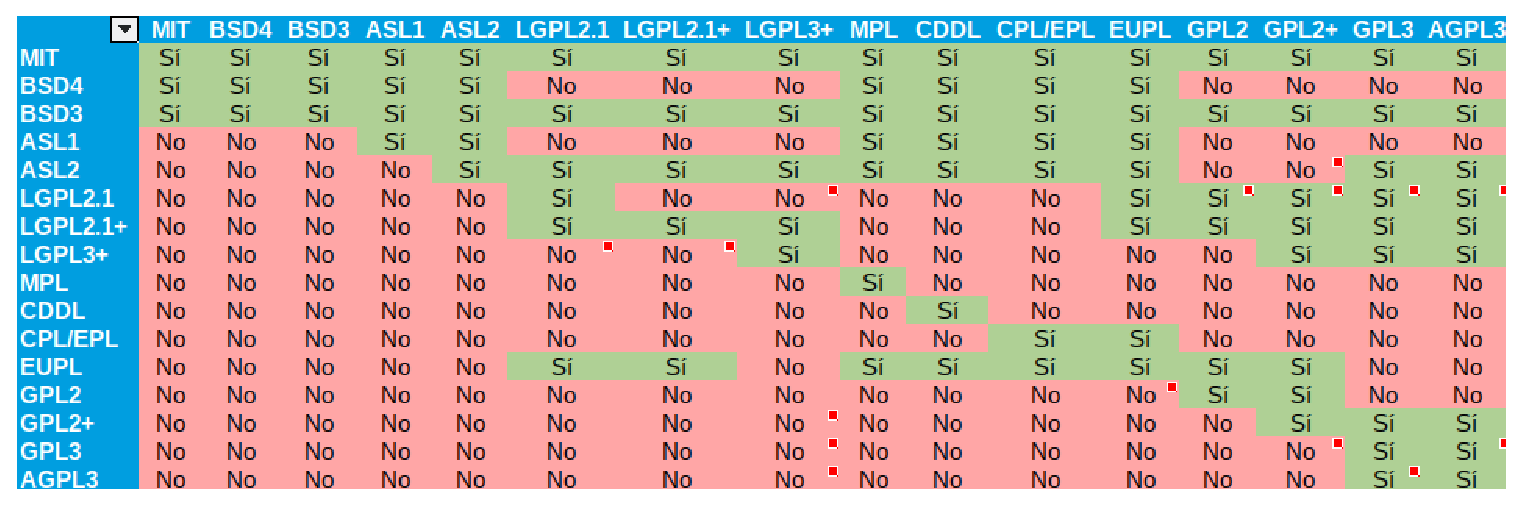
\includegraphics[scale=.5]{imagenes/matriz-estatica.eps}
\caption{Matriz de compatibilidad de licencias de paquetes de software estáticos.}
\end{subfigure}
\begin{subfigure}{\linewidth}
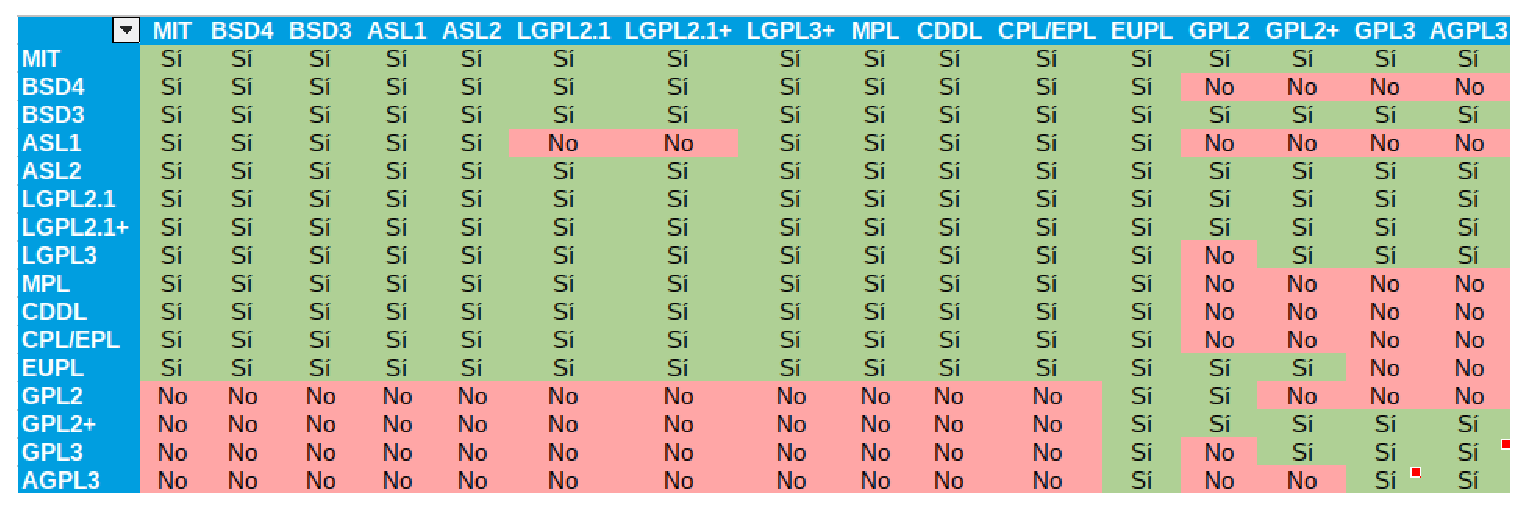
\includegraphics[scale=.5]{imagenes/matriz-dinamica.eps}
\caption{Matriz de compatibilidad de licencias de paquetes de software dinámicos.}
\end{subfigure}
\caption{Matrices de compatibilidad realizadas por el Centro Nacional de Referencia de Aplicación de las Tecnologías de la Información y Comunicación (CENATIC) en 2019}
\label{figMatriz}
\end{figure}

%\begin{itemize}
%\item {\bf Copyleft}
%Estrategia legal la cual permite hacer que el código sea libre, es decir, que pueda ser utilizado por cualquiera, modificarlo y mejorarlo para cualquier propósito, distribuir versiones originales y mejoradas con o sin lucro sin pedir permiso a nadie. Toda nueva versión o copia está basada en las mismas condiciones que el original.
%\item {\bf Copyright}
%Licencia más restrictiva, sólo el autor puede utilizarlo y si alguien quiere usarlo debe pedirle permiso al autor y pagarle. Si el software no tiene definida ningún tipo de licencia, adopta por defecto la copyright, cabe aclarar que su registro no es obligatorio. 
%\item {\bf Creative Commons}
%Determina cómo va a circular el software en internet, es decir, algunos autores pueden dar derechos a otras personas, son gratuitas y su registro no es obligatorio.
%\end{itemize}


%La característica peculiar de estas licencias se debe a que no poseen copyleft, ya que el trabajo derivado no tiene por qué mantenerse con el mismo régimen de derechos de autor que el original. Esto maximiza la libertad para quien recibe el software y quiere desarrollar algo derivado, permitiéndole elegir entre el amplio abanico de licencias existentes. No obstante, desde el punto de vista de los usuarios, esto se puede considerar como una restricción a su libertad, en el sentido de que el software propietario siempre restringe las libertades de los usuarios del mismo y las licencias permisivas, abren esta posibilidad. Los ejemplos más conocidos de este tipo de licencias son la Licencia MIT y la Licencia BSD.

%\section{Organismos}
%\begin{itemize}
%\item {\bf Fundación para el software libre(FSF) }
%Creada por Richard Stallman en 1985 con la finalidad de eliminar restricciones sobre copias, redistribución, entendimiento y modificación .Esto ayudó a promover el software libre, especialmente en el desarrollo de SO GNU. Actualmente se centra en asuntos legales, organizativos y promocionales del software libre. Stallman fue el creador del Copyleft 
%
%\item {\bf Open Source Initiative(OSI)}
%Creada por Bruce Perens y Eric S. Raymond en 1998 con la finalidad de promover el software libre. A fines del 1998 publicaron el código fuente de Netscape Communicator dadas las pérdidas y dura competencia con Internet Explorer de Windows. No podían competir ya que IE venía gratis con Windows, en cambio su producto era por separado y pago. Luego con la publicación del código fuente, hubo un grupo de personas que introdujo el término mercadotecnia que permitió levantar al software libre debido a que era más amigable. Gracias a este proyecto, surgen otros como Mozilla. 
%
%\item {\bf Proyecto Fedora}
%Comunidad responsable de la distribución de Fedora y otros proyectos. Es la fusión de Red Hat y el antiguo proyecto Fedora en 2003. El viejo Fedora desarrollaba paquetes para las viejas distribuciones de Red Hat (RHL 8 Y 9, FC1 Y 2).
%
%\item {\bf Directrices de software libre de Debian}
%Directrices que permiten ver si una licencia de software es una licencia de software libre y además si alguna licencia y software pueden incluirse en la distribución de Debian. Algunas de las directrices que podemos mencionar son:
%
%\begin{itemize}
%	\item Libre redistribución
%	\item Inclusión del código fuente
%	\item Permitir que las modificaciones y trabajos derivados sean hechos bajo la misma licencia
%	\item	Integridad del código fuente del autor, se debe permitir cuando menos la distribución de modificaciones por medio de parches
%	\item Sin discriminación de personas o grupos
%	\item Sin discriminación de áreas de iniciativa, como el uso comercial
%	\item Distribución de la licencia, se necesita aplicar a todo al que se redistribuya el programa
%	\item La licencia no debe ser específica a Debian, básicamente reiteración del punto anterior
%	\item La licencia no debe contaminar otro software
%\end{itemize}
%\end{itemize}
%%\newpage




%\section {Tipos de Licencias}
%El software no se vende, se licencia. Una licencia es aquella autorización formal con carácter contractual que un autor de un software da a un interesado para ejercer actos de explotación legales. Es decir, el software no se compra, sino que se adquieren una serie de derechos sobre el uso que se le puede dar. En las licencias de software libre esos derechos son muy abiertos y permisivos, apenas hay restricciones al uso de los programas. De ahí que ayude al desarrollo de la cultura. Pueden existir tantas licencias como acuerdos concretos se den entre el autor y el licenciatario. Desde el punto de vista del software libre, existen distintas variantes del concepto o grupos de licencias, las mismas pueden clasificarse en distintos grupos:\\


%\section{Papel de la FSF y OSI}
%
%{\bf Licencias de código abierto aprobadas por el OSI}
%El grupo OSI define y mantiene una lista de licencias de código abierto aprobadas por el mismo. OSI está de acuerdo con la FSF en la mayoría de las licencias de software libre, pero difiere en algunos de la lista de la FSF. Por ejemplo, se posiciona del lado de la definición de código abierto más que de la definición de software libre. Considera que las leyes del grupo licencias de software libre permisivas son una referencia de implementación de una licencia software libre. Esto es sus requerimientos para aprobar las licencias son diferentes.
%\\
%{\bf Licencias de software libre aprobadas por la FSF}
%La FSF, el grupo que mantiene la definición de software libre, mantiene una lista de licencias de software libre no exhaustiva.12 La FSF es una organización sin ánimo de lucro cuya misión es promover la libertad de los usuarios de los ordenadores y defender los derechos de todos los usuarios del software libre. Los desarrolladores de software libre garantizan que todo el mundo tenga los mismos derechos para sus programas, cualquier usuario puede estudiar el código fuente, modificarlo, y compartir el programa. Por el contrario, la mayoría del software lleva una nota que impide a los usuarios estos derechos básicos, dejando a los usuarios susceptibles a los deseos de sus propietarios y a la vulnerabilidad de ser vigilados. La FSF prefiere las licencias de software libre copyleft (share-alike) mejor que las licencias de software libre permisivas para la mayoría de los propósitos. En su lista distingue entre las licencias de software libre que son compatibles o incompatibles con el la GPL de copyleft de la FSF.
%
%%\newpage

%\section{Garantìas, condiciones y limitaciones brindadas por las licencias}
%\begin{itemize}
%\item Garantìas: Son aquellas características del software que son permitidas o autorizadas por la licencia.
%\begin{itemize}
%\item Usar: Se garantiza el uso del software
%\item Distribuir/Comerciar: Se permite su distribución y/o comercialización.
%\item Modificar: Se permite modificar características y funcionalidades del programa.
%\item Mejorar el programa y publicar las mejoras: Se pueden sugerir cambios y permitir que dichos cambios se lleven a cabo.
%\item Derechos de patente para sus contribuidores: Las patentes dependen de las leyes nacionales respecto a las licencias del software.
%\end{itemize}
%\item Condiciones: Son aquellas características que debe poseer todo software que derive del poseedor de la licencia
%\begin{itemize}
%\item Misma licencia: Debe mantener su licencia cuando se realicen modificaciones.
%\item Revelar fuente: Código fuente debe estar disponible cuando se distribuya el software
%\item Informar de licencia y copyright: Se debe poseer una licencia e informar del copyright junto con el software
%\item Red como medio de distribución: Se debe poder utilizar la red para recibir una copia del código fuente
%\item Cambios documentados
%\end{itemize}
%\item Limitaciones: Son todas las características que no garantiza la licencia respecto al uso del software.
%\begin{itemize}
%\item Responsabilidad: No se hacen responsables por el uso dado al software
%\item Garantía: No se provee ninguna garantía
%\item Uso de marca registrada: No garantiza el uso de la marca registrada
%\end{itemize}
%\end{itemize}



\chapter{Gestión de proyectos de software libre}
%\chapterauthor{Borello Agustín, Donato Alexis, López Marcos, Mattio Paolo, Vilardo Milena}

\section{Comunidades de software libre}

Dadas las características del software libre, raramente una única empresa desarrolla un paquete de software, como es habitual con el software privativo. El software libre es desarrollado en el seno de comunidades de software libre.

Una comunidad de software libre es un grupo de personas que cooperan entre sí para desarrollar, mantener o difundir uno o varios paquetes de software libre. Las personas en una comunidad pueden compartir una localidad o pueden estar distribuidas por el mundo. Una comunidad puede estar estrictamente organizada a través de reglamentos escritos y seguidos a rajatabla, o ser un grupo \emph{ad-hoc} sin demasiadas reglas. El liderazgo puede ser llevado adelante por una empresa, una organización, un grupo de personas o incluso una única persona.

A través del uso de Internet las comunidades de software libre se distribuyen alrededor del mundo y les permite estar compuestas por personas de distinto género, nacionalidad, conocimientos previos, formación académica, culturas, idiomas y motivaciones. Esta diversidad enriquece el desarrollo del software y ha permitido crear complejos productos informáticos, tales como sistemas operativos o compiladores, pero también hace compleja la gestión de los grupos de desarrollo.

Esta complejidad fue primero notada y analizada por Eric S. Raymond en una serie de artículos que luego se transformaron en su clásico libro ``La catedral y el bazar''~\cite{raymond01}, originalmente escrito en 1997, como un ensayo sobre la metodología de desarrollo del software de código abierto. En él analiza dos modelos de producción de software bien diferenciados. Por un lado, el modelo de desarrollo más hermético, planificado y vertical característico del software propietario, al que compara con la construcción de una catedral, donde cada pieza es cuidadosamente ensamblada por trabajadores bajo la guía de el/la o los/las arquitectos/as según un plan previamente trazado, sin que haya lugar a lanzar versiones de prueba antes de que haya llegado el momento de inaugurar la obra. Por el otro lado el modelo de desarrollo del kernel Linux, asimiliado por Raymond a un bazar persa\footnote{Si se quiere argentinizar la metáfora podríamos pensar en una de las ferias conocidas como Salada o ``saladitas''.} por su dinámica horizontal, caótica y bulliciosa, sin una planificación ni guía vertical estricta, formada por personas con diferentes objetivos y enfoques. Sorprendentemente, de ese caos aparente surge un sistema coherente, estable y útil, ya sea un bazar o el kernel de un sistema operativo. 

Raymond detectó ciertas características de liderazgo de Linus Torvalds que son fundamentales en el éxito de Linux y de otras comunidades de software libre. Una de ellas es lanzar versiones de prueba enseguida y a menudo. Bajo el lema ``libere pronto, libere a menudo y escuche a los usuarios'', el lanzamiento continuo de versiones mejoradas del sistema permite minimizar la redundancia de esfuerzos mediante la difusión rápida de correcciones ya realizadas, además de proveer un estímulo y recompensa constante a los usuarios (especialmente a los más ansiosos) que realizarán una constante revisión en cada versión, permitiendo detectar los errores de forma temprana y minimizando el costo de cada error.

Otra característica del liderazgo de Torvalds es delegar cuanto sea posible. Cualquier líder de una comunidad de software libre cuyo desarrollo dependa tan sólo de su cerebro va a estar siempre en desventaja frente al que sepa cómo crear un ambiente abierto y en evolución, en el cual tanto el desarrollo como la búsqueda de errores y las mejoras se confíen a cientos de personas.  

Tratar a los usuarios como colaboradores permite mejorar con rapidez y depurar eficazmente un programa. Esto a su vez permite hacer crecer la comunidad. Un número mayor de usuarios encuentra más errores debido a que añade muchas más formas diferentes de forzar el programa. Dada una base lo suficientemente amplia de probadores y colaboradores, casi todos los problemas se identificarán con rapidez y su solución será obvia para alguien.  

Para trabajar y competir con eficacia, quienes quieran desarrollar un proyecto en colaboración deben aprender a reclutar y motivar a la gente en base a intereses comunes y a conectar la individualidad de los/as colaboradores/as para llevarles a culminar objetivos difíciles solo alcanzables mediante una colaboración sostenida. Esto no quiere decir que la visión y la capacidad individual no importan. Los proyectos más exitosos de software libre son los que comienzan a partir de una idea y perserverancia de una persona pero que al mismo tiempo promueve la construcción de un grupo de trabajo con intereses comunes. 

\section{Roles en la comunidad}

Las personas que forman parte de una comunidad de software libre pueden cumplir varios roles: usuarios/as, diseñadores/as, desarrolladores/as, distribuidores/as, realizar soporte, traductores/as, instructores/as, entre otros. Sin embargo, existe una especie de categorización de los/as participantes: usuarios/as, contribuyentes\footnote{Para las personas que contribuyen al proyecto generalmente se usa el término en inglés \emph{contributors}, pero en este texto utilizaremos su versión en español.} y mantenedores/as. 

\begin{itemize}
\item{Usuario/a:} Quien comienza a utilizar un software libre con asiduidad se está uniendo a una comunidad de personas con un objetivo en común. Un/a usuario/a puede colaborar de muchas formas, tal como enviar informes de errores, realizar solicitudes de nuevas funcionalidades y promover el uso del software n ámbitos externos a la comunidad. Los/as usuarios/as proporcionan una muy necesaria retroalimentación a los contribuyentes y mantenedores.

\item{Contribuyente:} Un/a contribuyente no solo reporta un error sino que investiga las causas y propone una solución o incluso la implementa. Para ser contribuyente no es necesario saber progrmar, se puede contribuir con código o con documentación. Puede que tengan voz en la toma de decisiones.

\textbf{Mantenedor:} Los mantenedores son los/as líderes/sas del proyecto y comprometen mucho de su tiempo y energía en los proyectos. Normalmente, un mantenedor será el árbitro final de cualquier problema de diseño o codificación que surja dentro del proyecto. Es un título de prestigio, pero requiere una inversión superior en tiempo y esfuerzo. Son quienes deciden los pasos siguientes del proyecto y la orientación general de la comunidad.
\end{itemize}

Para pasar de usuario/a a contribuyente, e incluso avanzar en la complejidad e importancia de las contribuciones a un proyecto, existe un conjunto de pasos que se siguen, usualmente en forma escalonada, ya que cada paso requiere de mayor conocimiento del código del proyecto.

\begin{itemize}
     \item Instalar el software en la computadora personal.
     \item Usar el software.
     \item Si es el caso, instalar el software en un servidor Web. 
     \item Participar de los foros de discusión.
     \item Promover el software en ámbitos externos a la comunidad.
     \item Realizar tareas de instrucción sobre el uso del software.
     \item Traducir, mejorar o crear documentación.
     \item Verificar las distintas versiones y reportar errores.
     \item Modificar el código para personalizar una operación o corregir un error.
     \item Crear un módulo para extender el software con una funcionalidad.
     \item Aportar un módulo para ser incorporado en la versión oficial del proyecto.
\end{itemize}

El primer paso para pasar de usuario a involucrarse más personalmente en un proyecto de software libre es contactar a los mantenedores personalmente o a través de los foros en línea de la comunidad, ofrecer sus servicios y preguntar qué es lo que la comunidad está necesitando más en ese momento.

%Se puede deducir que existe una gran influencia universitaria en el Software Libre. Esto no es de extrañar, ya que, como se ha podido ver en el capítulo de historia, el Software Libre –{\bf antes incluso de llevar esta denominación}– ha estado íntimamente ligado a las instituciones educativas superiores. Aún hoy, el verdadero motor del uso y expansión del Software Libre siguen siendo las universidades y los grupos de usuarios estudiantiles. No es, por tanto, de extrañar que más de un 70\% de los desarrolladores cuenten con una preparación universitaria. El dato tiene mayor importancia si tenemos en cuenta que del 30\% restante muchos no son universitarios porque todavía están en su fase escolar. Aun así, también tienen cabida –{\bf y no por ello son menos apreciados}– desarrolladores que no han accedido nunca a estudios superiores, pero que son amantes de la informática.


\section{Toma de decisiones}

Arriba hemos mencionado que tanto contribuyentes como mantenedores/as aportan a la toma de decisiones dentro de la comunidad. En particular, el involucramiento en la toma de decisiones dependerá de varios factores, tanto personales como del proyecto.

\begin{itemize}
     \item Experiencia e involucramiento de la persona en la comunidad: A más tiempo y dedicación a la comunidad, mayor será el nivel de responsabilidad y poder de toma de decisiones de una persona.
     \item Nivel de impacto de la decisión a tomar en el proyecto: Las decisiones más importantes son tomadas por un grupo de personas a cargo, generalmente decisiones respecto al \emph{core}. Para decisiones de menor impacto las discusiones son menos, como la mejora de características de un paquete.
     \item Pertenencia a diferentes áreas del proyecto: Dentro de un proyecto de software existen diferentes áreas con (usualmente) diferentes responsables, por lo que ellos/as son quienes pueden tomar decisiones y guiar a sus miembros para llevarlas a cabo.
\end{itemize}

Más allá de las características personales de los/as miembros de la comunidad y de las características técnicas del software desarrollado, existen diferentes estilos de toma de decisiones utilizados por las comunidades de software libre.

\begin{itemize}
\item Monárquico: Donde las decisiones mas importantes del proyecto son llevadas a cabo por una persona o líder (por ejemplo, Linux).
\item Comunitaria: Se toman las decisiones de manera democrática y no existe una persona o rol central en el proyecto (por ejemplo, PostgreSQL).
\item Corporativa: El liderazgo del proyecto lo tiene una empresa privada o una fundación sin fines de lucro, y son ellas quienes toman las principales decisiones de manera formal (por ejemplo, Fedora de la empresa Red Hat o Firefox de la Fundación Mozilla).
\end{itemize}

Cabe destacar que entre los estilos Monárquicos y Comunitarios existe todo un espectro de posibles estilos intermedios, donde el número de quienes pueden participar (con voz o voto) en la toma de decisiones se va ampliando desde una única persona en el Monárquico a toda la comunidad en el Comunitario.

Además, otro aspecto importante en la toma de decisiones dentro de un proyecto de software libre es que en general el mérito dentro de la comunidad es tenido en cuenta. Aquellas personas que han contribuido de manera importante y que han ganado credibilidad con respecto a sus habilidades dentro de la comunidad son las que serán tenidas en cuenta a la hora de tomar una decisión, sea cual fuera la estructura de un proyecto.

\section{Comunicaciones en la comunidad}

Debido a la naturaleza de los proyectos de software libre y a que los participantes de estos pueden trabajar desde ubicaciones muy distantes, cobran una gran importancia los distintos medios de comunicación que se utilizan, tanto para coordinar las actividades de la comunidad, como para comunicar al exterior las novedades del proyecto.

La comunicación se hace principalmente a través de Internet, utilizando las siguientes herramientas.

\begin{itemize}
     \item Sitio web: permite transmitir la información del proyecto al público en general y dar a conocer actualizaciones, decisiones y problemas.
     \item Listas de correo electrónico: permite la comunicación y discusión horizontal en la comunidad y es el más sencillo de implementar, pero es el más lento debido a que es asincrónico.
     \item Mensajería instantánea: sirven para la publicación de problemas, proponer soluciones y llevar adelante discusiones, permitiendo la participación sincrónica y horizontal.
\end{itemize}

La moderación de estos espacios de discusión es un tema muy importante en una comunidad de software libre y la falta de control puede llevar a que se tengan experiencias personales y profesionales muy negativas que lleven a la disgregación de la comunidad.

%\section{¿Cómo se hace disponible el codigo fuente del proyecto?}
\section{Herramientas de gestión}
%código fuente y sistemas de gestión de errores

Existen dos canales de comunicación fundamentales en una comunidad de software libre que lleva adelante el desarrollo de un proyecto de software: el código fuente y las descripciones de \emph{issues} (con esta palabra en inglés describimos tanto a los errores detectados como a las mejoras propuestas o a las  nuevas funcionalidades deseadas para un software). Para su gestión existen herramientas digitales que permiten ordenar su uso, modificación y almacenamiento.

El código fuente de un software libre es requerido por definición y también para poder hacer el desarrollo a través de un grupo, generalmente distribuido globalmente. Para esto se utilizan servicios de infraestructura de alojamiento en la web, que no solo dan posibilidad de tener un lugar en el internet donde se puede tener acceso a las fuentes del proyecto, sino que brindan herramientas que facilitan la gestión del proyecto, tales como el manejo de permisos de modificación, publicación de \emph{issues}, revisión de código propuesto y el almacenamiento de versiones anteriores.

En la actualidad los servicios más populares para este fin (aunque no son exclusivos para proyectos de software libre, ya que otros grupos o empresas pueden almacenar su código allí) son GitHub\footnote{GitHub: \url{https://github.com/}} y GitLab\footnote{GitLab: \url{https://gitlab.com/}}.

Estos servicios proveen, como dijimos, un conjunto completo de herramientas de gestión. En particular herramientas para gestión de \emph{issues} y para control de versiones. Un \emph{issue} es un problema o error detectado en el software o una tarea para realizar, ya sea una mejora, una corrección o el agregado de alguna funcionalidad al software. Dijimos previamente que uno de los roles de los/as usuarios/as avanzados/as en una comunidad de software libre era detectar errores en el software. A través de un sistema de gestión de \emph{issues} los/as usuarios/as pueden reportar dichos errores en una forma normalizada, que exige la información mínima necesaria para que el error pueda ser reproducido y una solución propuesta por los/as contribuyentes. Además, información extra puede ser agregada o discutida por otros/as miembros de la comunidad, e incluso se pueden agregar rótulos que indican la prioridad o el tipo de error (por ejemplo, se los puede rotular como ``crítico'' o ``adecuado para principiante''). Los repositorios de código mencionados proveen sus propios sistemas de gestión de \emph{issues}, aunque también existen sistemas independientes, como por ejemplo Bugzilla\footnote{Bugzilla: \url{https://www.bugzilla.org/}}.


Para cualquier proyecto de software, es muy importante la implementación de un sistema de control de versiones para poder gestionar los diversos cambios que se realizan sobre sus componentes. Esto cobra una importancia aún mayor en proyectos de software libre, ya que la heterogeneidad de su comunidad de contribuyentes requiere que las modificaciones al código tengan un control más estricto. Aunque existen muchos sistemas de control de versiones, tales como Subversion\footnote{Apache Subversion: \url{https://subversion.apache.org/}} (o SVN) y Mercurial\footnote{Mercurial: \url{https://www.mercurial-scm.org/}}, el más difundido en la actualidad es Git\footnote{Git: \url{https://git-scm.com/}}, creado originalmente por Linus Torvalds y que es la base de los dos repositorios mencionados (de ahí sus nombres).


\section{Control de calidad}

El enfoque actual para asegurar la calidad del software es utilizar procedimientos estándares durante el proceso de desarrollo, guiados por equipos de aseguranza de la calidad del software (QA, por las siglas de \emph{Quality Assurance}). Implementar estos estándares es un desafío para las comunidades de software libre, ya que usualmente siguen un modelo horizontal al estilo bazar.

Algunas falencias comunes son la falta de pruebas unitarias asociadas al código presentado para su inclusión en el software siendo desarrollado, la inexistencia de ciclos de testing llevados adelante por un grupo o departamento de calidad independiente de los/as desarrolladores/as y la baja calidad de los reportes de defectos, con información incompleta o poco precisa, ya que usualmente son escritos por usuarios/as sin formación en informática. Actualmente, gracias al auge de los procesos de integración continua y a la integración de herramientas que los implementan en los repositorios, se han mejorado los primeros dos aspectos mencionados, ya que se exige que el código incluya pruebas unitarias y se ejecutan conjuntos de pruebas en forma automática antes de aprobar la solicitud de inclusión del código en el proyecto (usualmente llamado, en el ambiente de Git, \emph{pull request}). 

Respecto al bajo nivel de los reportes de defectos o \emph{issues}, debe tenerse en cuenta que son el resultado de dos características positivas del software libre: el lanzamiento continuo de versiones mejoradas (las cuales aún tienen defectos conocidos o pueden tener nuevos defectos no detectados antes de su lanzamiento) y el involucramiento de toda la comunidad en la búsqueda de errores en el software. El problema puede minimizarse dedicando tiempo de los/as contribuyentes y mantenedores/as a la revisión detallada de los defectos reportados, de modo que ningún defecto sea considerado como aceptado hasta que un/a desarrollador/a experimentado/a lo revise, reproduzca y apruebe.



\chapter{Modelos de negocio con software libre}

Ya debe haber quedado claro que el software libre no es necesariamente gratis, aunque, como dijimos previamente, el costo del código tiende a cero, por lo que el modelo de negocios tradicional en la industria del software no puede aplicarse a este tipo de software. Otra característica que surge del modelo de desarrollo de software libre es que es imposible, a diferencia del software propietario, obtener ventajas abusivas por posición dominante (característica conocida comúnmente como ``monopolio''), ya que el código fuente está disponible para cualquier persona o empresa, y ante abusos del grupo de desarrollo se puede producir una división (a veces denominada \emph{fork}) y generar un producto con las mismas características que el original. 

En este capítulo presentaremos algunos de los modelos de negocios que pueden utilizarse en el marco del software libre o de fuentes abiertas, haciendo la aclaración que algunos de ellos pueden superponerse o combinarse en algunos proyectos.

\section{Financiación pública}

Siguiendo un modelo similar al de la financiación de la investigación básica, las instituciones públicas o fundaciones sin fines de lucro pueden proveer apoyo económico a proyectos de software libre. Según las características del proyecto y los objetivos de la institución financiante, puede que la institución participe o no en la gestión del proyecto y desarrollo del software.

Usualmente no busca recuperar la inversión, pero tiene objetivos claros. Por ejemplo, favorecer cierta industria, promover cierta tecnología o estándares, desarrollar herramientas de bajo costo para instituciones públicas, facilitar el acceso a tecnología, etc.

Un caso cercano de este tipo es el desarrollo del sistema operativo Huayra, una distribución GNU/Linux, que es financiado por el gobierno argentino a través de un equipo de desarrollo propio\footnote{Huayra GNU/Linux: \url{https://huayra.educar.gob.ar/}}. Esta distribución, y algunas aplicaciones desarrolladas por el mismo equipo, es incluida en las computadoras del Plan Conectar Igualdad, que distribuye computadoras portátiles a estudiantes de escuelas secundarias públicas de todo el país\footnote{Plan Conectar Igualdad: \url{https://conectarigualdad.edu.ar/}}.

\section{Financiación privada}\label{sec:finPrivada}

Algunos proyectos de software libre son llevados a cabo o financiados por empresas, es decir, instituciones con fines de lucro. En forma similar a la financiación anterior, tanto los objetivos como el involucramiento de la empresa en la gestión y desarrollo del proyecto pueden variar.

Un ejemplo interesante de estos dos tipos de financiación, y de cómo esta va variando a lo largo de la vida de un software, es el de la suite de oficina OpenOffice: el software privativo llamado StarOffice, fue adquirido en 1999 por la empresa Sun Microsystems para uso interno, pero en 2002 lo liberó como software libre con el nombre de OpenOffice para competir con la suite Microsoft Office y promover la utilización del estándar libre de documentación ODF (siglas de \emph{Open Document Format}. En 2010 la empresa fue adquirida por Oracle Corporation y al año siguiente se informó que no se continuaría financiando el proyecto OpenOffice, el cual se donó a la Fundación Apache, que lo sigue desarrollando bajo el nombre de Apache OpenOffice\footnote{Apache OpenOffice: \url{https://www.openoffice.org/es/}}. Mientras tanto, un grupo independiente de la comunidad realizó un \emph{fork} y creó la fundación The Document Foundation, la cual, en base al código de OpenOffice, desarrolla actualmente la suite LibreOffice\cite{watkins18}\footnote{LibreOffice: \url{https://es.libreoffice.org/}}.

En las últimas décadas han surgido cooperativas (empresas gestionadas por sus trabajadores\footnote{Formalmente una cooperativa es una asociación autónoma de personas que se han unido
voluntariamente para hacer frente a sus necesidades y aspiraciones económicas, sociales o culturales comunes por medio de una empresa de propiedad conjunta y democráticamente controlada.}) dedicadas a la tecnología basada en software libre o que desarrollan software libre. Lo mencionamos como un caso especial debido a que la filosofía del movimiento de software libre y los principios cooperativos tienen muchos puntos en común, tales como la pertenencia abierta y voluntaria a la comunidad o empresa, el control horizontal por parte de sus miembros, el compromiso con la comunidad, el compartir el conocimiento y el aporte del saber de cada miembro de la comunidad\cite{monk14}.

\section{Financiación por quien necesita mejoras}

Cuando un/a usuario/a o empresa requiere mejoras o funcionalidades específicas en un software libre puede financiar a un grupo (de la comunidad o ajeno a ella) para que las desarrolle. Cabe destacar que si el software mejorado resultante es para uso interno de la empresa no es requisito la redistribución libre del código generado, aunque el original tenga una licencia robusta. Sin embargo, si el software se redistribuye solo o como parte de un producto o servicio, una licencia robusta exigirá que la mejora (aún siendo pagada por la empresa) sea distribuida con la misma licencia que el código original. También es costumbre compartir el nuevo código aunque no sea un requisito legal, como aporte a la sociedad y en agradecimiento por el software original.

Este tipo de financiación permite que software desarrollado globalmente beneficie al mercado local, ya que usualmente se contrata a equipos de trabajo locales por una cuestión de cercanía, afinidad cultural y mayor simplicidad en los procesos comerciales y legales.

Una variación de este tipo de financiación es el aporte de tiempo de trabajo de desarrolladores/as de una empresa a un proyecto de software libre. Un grupo de desarrolladores/as de una empresa dedica su tiempo de trabajo, total o parcial, a desarrollar componentes o realizar mejoras a un software libre, formando parte de la comunidad. Este tiempo es pagado por la empresa como parte del sueldo de los/as desarrolladores/as. Este fue el caso de Corel, que en 1999 dedicó un equipo de ingenieros/as al proyecto Wine\footnote{Wine (\emph{Wine Is Not an Emulator}) es un software libre que implementa las API de Microsoft Windows en Linux, permitiendo que  aplicaciones desarrolladas para Windows se ejecuten en un sistema Linux sin necesidad de ser recompiladas. \url{https://www.winehq.org/}} para que le agregaran funcionalidades que permitiría que las aplicaciones de Corel, tales como WordPerfect, CorelDRAW y Quattro Pro, correr en Linux en forma eficiente y sin necesidad de reescribir el código de las aplicaciones~\cite{corel99}.

\section{Financiación por consultoría}

Este tipo de negocios es similar al anterior, pero generalizado a cualquier tipo de actividad que requiera el cliente. Tanto puede ser realizar mejoras al software (arreglo de errores específicos, agregado de funcionalidades) como análisis para determinar si el software es el adecuado para la empresa o actividades de instalación de software particularmente complicado o en ambientes complejos.

El fundamento de este modelo de negocios es que las empresas usuarias de software libre generalmente ante un problema del software no pueden depender de los tiempos de la comunidad sino que requieren una solución inmediata. El firmar acuerdos de servicio técnico con empresas proveedoras le permite garantizar ciertos tiempos de respuesta adecuados para asegurar la continuidad del negocio.

Este es el enfoque de negocios de muchas de las empresas basadas en software libre más exitosas. El mayor ejemplo de esto es Red Hat\footnote{Red Hat: \url{https://www.redhat.com/es}}, cuyo servicio de consultoría basado en una distribución del sistema operativo GNU/Linux, comenzando en 1993 la llevó a ser una empresa valuada en 33 mil millones de dólares, precio al cual la adquirió IBM en 2018.
 
\section{Financiación por servicios web}

Recientemente, y dependiendo de sus características, muchos proyectos de software libre ofrecen tanto una versión para instalar en los equipos de los/as usuarios/as como una versión en la nube, que provee servicios web con ciertos esquemas de pago (puede haber un servicio básico gratuito y mayores precios según los servicios provistos). Lo que se cobra en este caso no es el software, sino los servicios web (almacenamiento, gestión de usuarios, etc.).

Cabe notar que una ventaja de este enfoque comercial es que el/la usuario/a no necesita estar pendiente de las nuevas versiones, el software en la web se actualiza a medida que aquellas van siendo liberadas. Por otro lado, al ser software libre, si el/la usuario/a no está conforme con los servicios provistos puede descargarlo e instalarlo en sus equipos o en los equipos de un proveedor de servicios de nube y continuar usándolo sin mayores costos.

Un ejemplo de este tipo de negocio es Moodle\footnote{Moodle: \url{https://moodle.org/}}, la plataforma de gestión de clases que utilizamos en esta asignatura. La instancia que utilizamos está instalada en los servidores del centro de cómputos de la UTN-FRC, pero instituciones que no tengan estas facilidades pueden adquirir diferentes planes y utilizar Moodle en la nube. En la Fig.~\ref{figMoodle} se muestran los diferentes planes al día de hoy. 

\begin{figure}[h!]
\centering
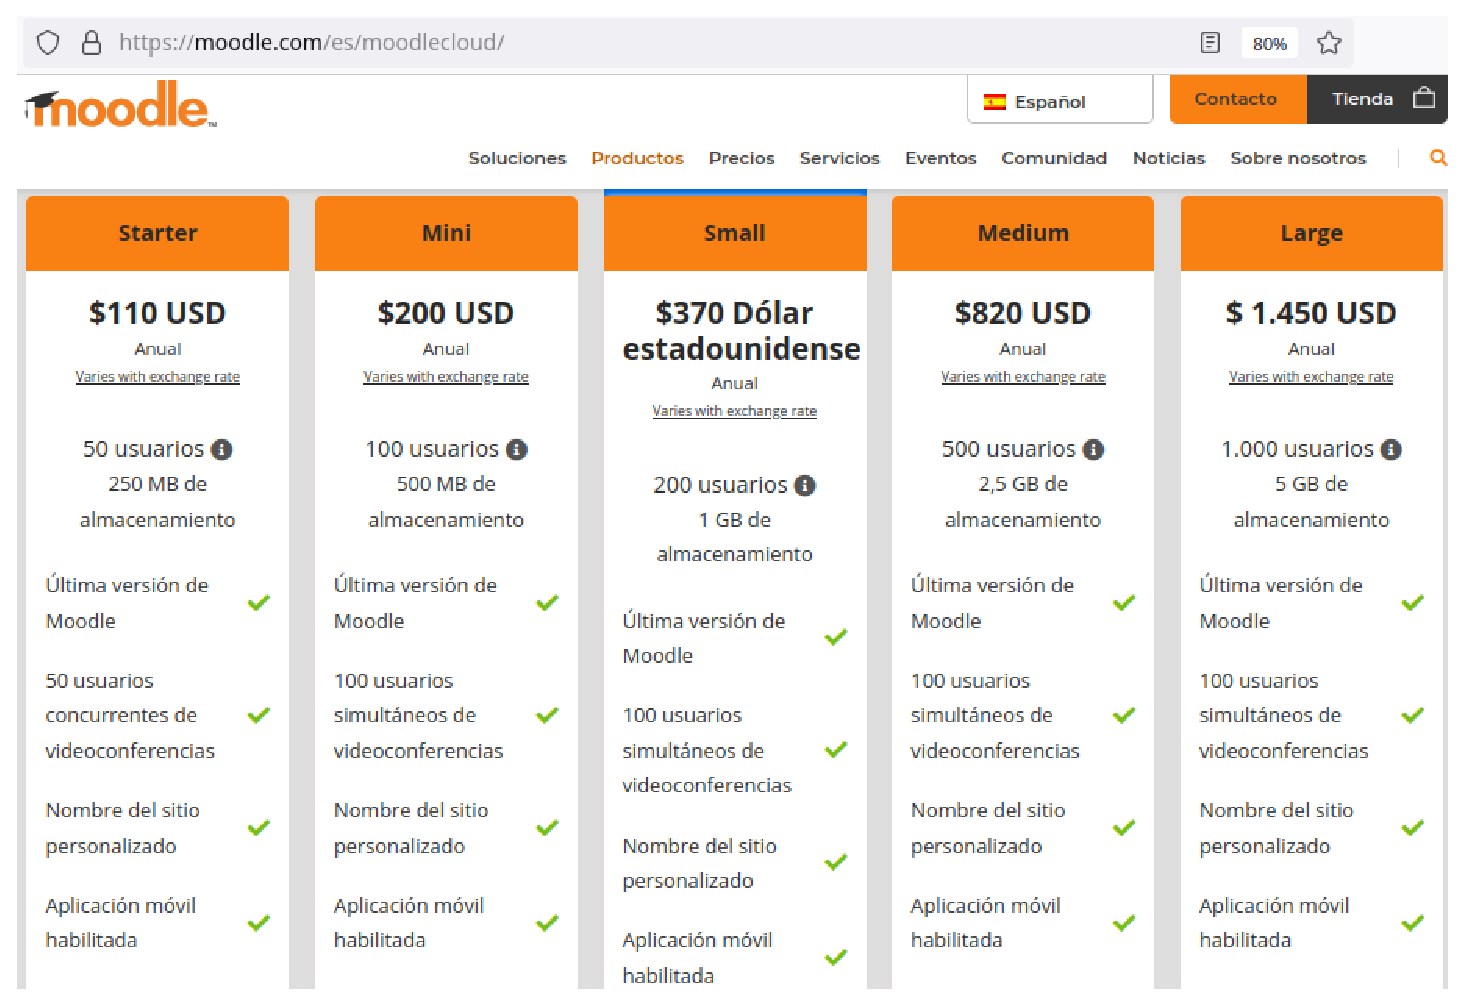
\includegraphics[scale=.5]{imagenes/moodle.eps}
\caption{Planes de servicio de Moodle en la nube. Precios en dólares al 23/02/2022.}
\label{figMoodle}
\end{figure}


\section{Financiación por productos relacionados}

Ya que no es razonable vender el código, una fuente de financiación de proyectos libres es la venta de productos asociados, ya sean tangibles o intangibles.

\begin{itemize}
\item {\bf \emph{Merchandising}:} Es común la venta de remeras, gorras, calcos y otro material sobre proyectos o comunidades de software libre. Para que los fondos obtenidos de esta manera beneficien a la comunidad que desarrolla el software es usual que la marca, nombre y/o logo del proyecto estén protegidos legalmente. Por ejemplo, Linux es una marca registrada de Linus Torvalds y Firefox es marca registrada de la Mozilla Foundation, así como el logo del navegador.

\item {\bf Formación:} Cursos, entrenamiento, manuales y libros sobre software libre también son fuentes de ingresos para las comunidades de software libre. Aunque cualquier persona o empresa puede desarrollar actividades de formación sobre un proyecto de software libre, usualmente quienes están involucrados en la comunidad están en ventaja para hacerlo, ya que poseen un conocimiento profundo del software en cuestión.
 
\end{itemize}

Como ejemplo de esto último mencionamos en particular a la editorial O’Reilly, que publica libros sobre diferentes proyectos de software libre, beneficiando generalmente a sus creadores originales. Debe notarse, además, que muchos de sus libros a su vez tienen licencias libres\footnote{O'Reilly Open Books: \url{https://www.oreilly.com/openbook/}}.

\section{Licenciamiento múltiple}

En algunos casos, para financiar el proyecto libre el producto de software se distribuye bajo dos licencias o más, siendo al menos una de ellas libre y las otras propietarias. Generalmente las versiones bajo licencia propietaria tienen funcionalidades que la versión libre no tiene (pasado un tiempo esas funcionalidades se agregan a la versión libre, pero quienes pagan por la licencia propietaria pueden acceder antes a estas funcionalidades).

Usualmente las versiones bajo licencia propietaria incluyen servicios de consultoría y tiempos de respuesta rápidos a solicitudes del/la usuario/a.

Un clásico ejemplo, entre muchos, es la base de datos MySQL\footnote{MySQL: \url{https://www.mysql.com/}} que utiliza la licencia GPL para su \emph{Community Edition} y una licencia propietaria de Oracle para su versión comercial.

\section{Financiamiento por donaciones}

Algunos proyectos de software libre se financian (al menos parcialmente) a través de donaciones de particulares y empresas. Para facilitar este tipo de financiación se han creado fundaciones que gestionan las finanzas del proyecto (como vimos en la sección~\ref{sec:finPrivada}), aunque esto no es requisito y dependerá de los montos de donaciones que se manejan en cada proyecto.

\section{A modo de cierre}

Hemos visto en este capítulo diferentes modos de financiar (total o parcialmente) un proyecto de software libre. Cabe aclarar que estos modelos de negocios no son excluyentes, muchas comunidades se financian a través de una combinación de estos.



%\section{Impacto sobre las Situaciones de Monopolio}
%
%
%Cualquier iniciativa dedicada a romper una situación donde un producto domina claramente el mercado estará destinada a producir más de lo mismo: si tiene éxito, vendrá otro a ocupar ese hueco y en breve habrá otro dominante. Solo los cambios tecnológicos producen durante un tiempo la inestabilidad suficiente como para que nadie domine claramente.
%El problema no es que haya un producto dominante, sino que haya solamente una empresa que lo ofrezca al mercado. El SW libre ofrece la alternativa a esa situación.
%Lo saludable es que cualquiera sea el producto, muchas empresas puedan competir para proporcionarlo, mejorarlo, adaptarlo y ofrecer servicios alrededor de él.
%
%\subsection{Elementos que favorecen a los productos dominantes}
%
%{\bf Formato de datos:  } cuando mucha gente utiliza un formato de dato dado, la presión para usarlo es enorme.
%
%{\bf Cadenas de distribución: } cuando el producto es dominante es fácil su distribución porque todas las cadenas lo buscan para poder ofrecerlo. Si el producto es minoritario le resulta difícil acceder a su comercialización y llegar a los usuarios.
%
%{\bf Marketing: } el boca a boca es una gran propaganda, cuando son muchos los que lo usan. 
%
%{\bf Inversión en formación: } una vez aprendido el uso de una herramienta, se está muy motivado para no cambiar. Además, usualmente esa herramienta es la que domina, por lo que es más fácil encontrar material y personas que ayuden a aprenderla.
%
%{\bf Software preinstalado: } el usuario lo quiere. Además, el SW que viene preinstalado es el más utilizado.
%
%\subsection{El mundo del software propietario}
%
%En este mundo, la aparición de un producto dominante en un segmento cualquiera equivale a un monopolio por parte de la empresa que lo produce.
%La empresa tiene gran control sobre el producto, ellos marcan su evolución, su calidad, etc. 
%Esta situación hace aparecer los peores efectos económicos del monopolio, entre ellos la falta de motivación de la empresa líder para acercar el producto a las necesidades de sus clientes, ya que están cautivos.
%
%\subsection{La situación del software libre}
%
%Con el SW libre, un producto dominante no se traduce en monopolio de la empresa. Cualquier empresa puede trabajar en él, mejorarlo, adaptarlo a las necesidades del cliente y ayudar a su evolución. Muchos querrán trabajar en esta mejora y si la empresa que lo desarrolló en primera instancia quiere permanecer en el negocio tendrá que competir contra todas ellas y estará muy motivada para hacer evolucionar al producto. Naturalmente tendrá la ventaja de un mejor conocimiento del programa. 
%Los usuarios retoman el control.
%Como ejemplo de productos libres que son dominantes en su sector se puede nombrar Apache y las distribuciones de GUN/Linux.
%
%\subsection{Estrategias para constituirse en monopolio con software libre}
%
%Son estrategias comunes a otros sectores económicos, pero una es específica del mercado del SW: {\bf la aceptación de productos certificados por terceros.}
%Cuando una empresa quiere distribuir SW que funcione en combinación con otras aplicaciones, es común “certificar” la combinación. El fabricante se compromete a ofrecer servicios (actualización, soporte, resolución de problemas) sólo si el cliente está usando el producto en un entorno certificado por él. Si en este segmento la certificación es importante, estamos ante una nueva situación de monopolio.
%Las situaciones monopólicas no son fáciles de conseguir, y para conseguirlas se debe utilizar mecanismos “no informáticos”.
%
%


\chapter{Sistemas operativos de software libre}
%\chapterauthor{Benito Federico, Filardo Juan, Simoncelli Fabricio, Ríos Julieta, Ulla Gonzalo}

Un sistema operativo libre es, como todo software libre, aquél que puede ser copiado, estudiado, modificado, utilizado libremente con cualquier fin y redistribuido con o sin cambios o mejoras.
En este capítulo presentaremos algunos sistemas operativos libres y su historia, ya que son fundamentales en el \emph{stack} de software libre.

\section{Historia de los SO derivados de Unix}

Los primeros sistemas operativos surgen en la década de 1950, pero la revolución es este campo ocurre durante los '60. Allí aparecen conceptos como sistemas multitareas, multiusuarios, multiprocesadores y de tiempo real. En esta década emerge Unix, base de la mayoría de los sistemas operativos libres actuales.

Unix fue desarrollado desde 1969 por Ritchie, Thompson y McIlroy en los laboratorios Bell de AT\&T. Es un sistema operativo portable, multitarea y multiusuario originalmente destinado a mainframes. Se caracteriza por poseer un núcleo monolítico y estar originalmente escrito en C (lenguaje a su vez creado por Ritchie).

Debido a que un fallo judicial antimonopolio impedía a la empresa de telecomunicaciones AT\&T comercializar software, Unix no fue comercializado inicialmente y se distribuía a las universidades con una licencia muy laxa. A partir de estas versiones de Unix varias universidades crearon sus propios sistemas operativos, el más exitoso y duradero es el sistema operativo libre BSD (por \emph{Berkeley Software Distribution})\footnote{BSD: \url{https://www.bsd.org/}} realizado en la Universidad de Californa en Berkeley. 

Por el problema de licencias mencionado y sus fortalezas técnicas, muchos sistemas operativos, libres o privativos, son variaciones de Unix. En la Fig.~\ref{figDerivUnix} vemos el árbol de sistemas operativos derivados de Unix, identificados por color según su esquema de licenciamiento: verde para fuentes abiertas, naranja pálido para los sistemas mixtos, con fuentes compartidas (pero no necesariamente abiertas o libres), y rosa para los sistemas privativos.

\begin{figure}[h!]
\centering
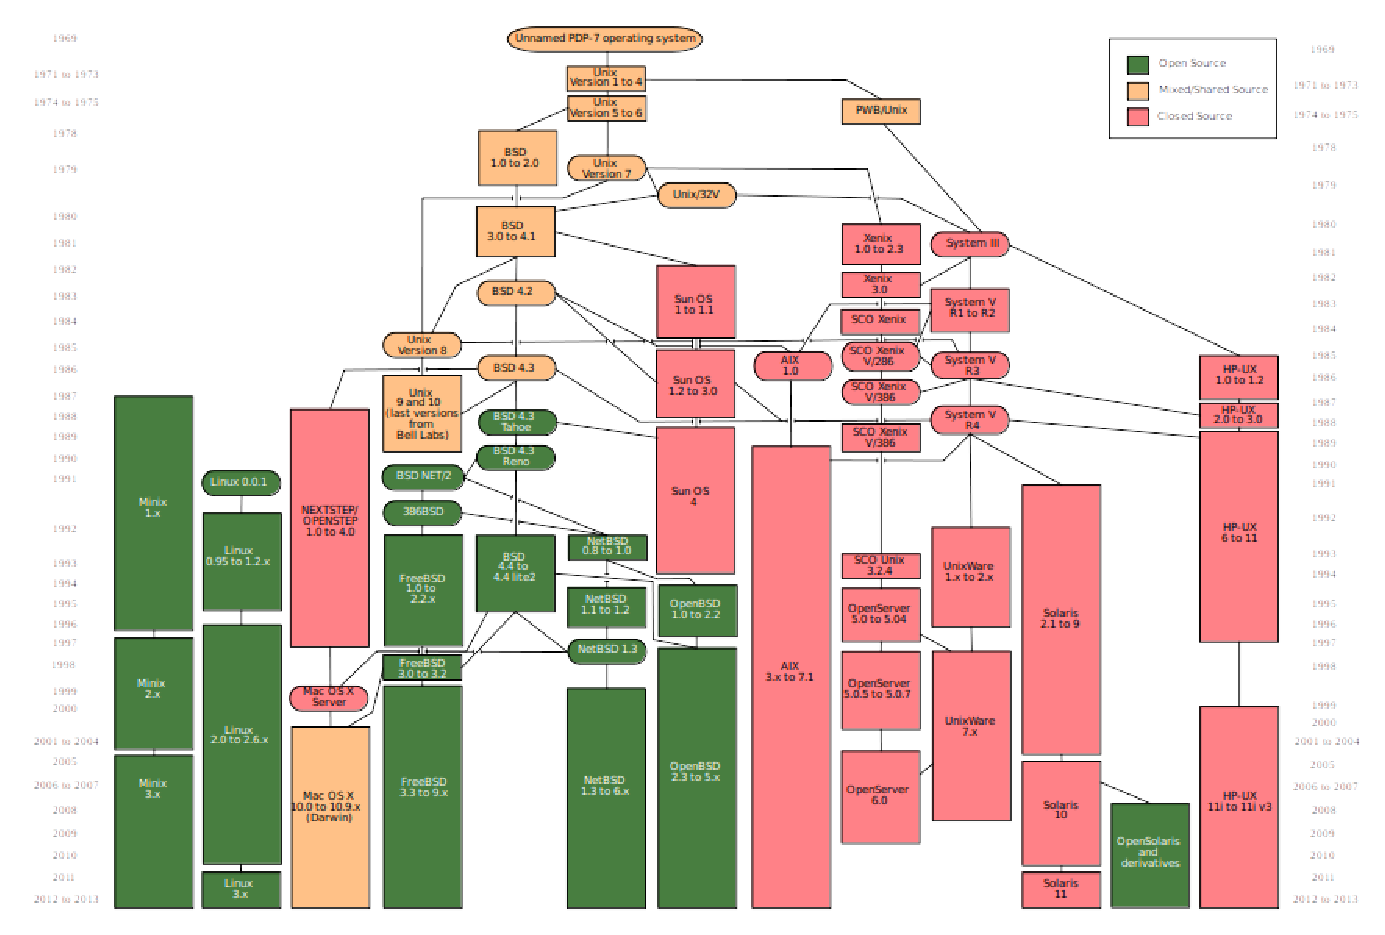
\includegraphics[scale=.5]{imagenes/arbolUnix.eps}
\caption{Sistemas operativos derivados de Unix.}
\label{figDerivUnix}
\end{figure}

Interesantemente, en las columnas de la izquierda podemos ver dos linajes derivados pero que no están conectados por una línea a Unix: Minix y Linux. La falta de conexión indica que, aunque derivados de Unix en el sentido de que siguen el estándar POSIX\footnote{Esto quiere decir que se comportan igual que Unix, respondiendo a los mismos comandos de la misma forma. Estándar POSIX: \url{https://es.wikipedia.org/wiki/POSIX}}, el código de estos sistemas operativos fue escrito desde cero. 

En el caso particular de Minix (llamado así por ser un MINI-uniX), este sistema operativo está basado en la tecnología de \emph{microkernel}, a diferencia de todos los otros sistemas de este árbol, que presentan un kernel monolítico. Otra particularidad de Minix es que durante mucho tiempo el código fuente impreso era parte del libro ``Sistemas Operativos: Diseño e Implementación''~\cite{tanenbaum87}, lo que hacía que el libro tuviera una longitud de 719 páginas. Ediciones posteriores eran acompañadas por versiones de Minix en diskettes o CD. Actualmente la versión 3 se puede obtener de un sitio web oficial\footnote{Minix 3: \url{http://www.minix3.org/}}.
	
\section{Distribuciones Linux}

Como se mencionó en el capítulo~\ref{capIntro}, los sistemas operativos libres más exitosos actualmente están basados en el núcleo (o \emph{kernel}) Linux. En vez de hablar de sistemas operativos diferentes, usualmente se los menciona como una ``distribución Linux'' (coloquialmente llamada \emph{distro}): una distribución es un sistema operativo basado en el núcleo Linux que incluye paquetes de software extra que le permiten satisfacer las necesidades de un grupo específico de usuarios. 

Una distribución Linux contiene típicamente el núcleo, herramientas y bibliotecas, software adicional, documentación, un sistema de ventanas, un administrador de ventanas y un entorno de escritorio. La mayor parte del software incluido es libreo o de fuentes abiertas y, por lo tanto, distribuido en binario compilado y en código fuente, permitiendo a sus usuarios modificar o compilar el código fuente original si lo desean. Muchas distribuciones incorporan software privativo, no disponible en forma de código fuente.

Si las distribuciones incluyen habitualmente las bibliotecas y herramientas del proyecto GNU, se la denomina GNU/Linux\footnote{La FSF (\textit{Free Software Foundation}) promueve el nombre de GNU/Linux para el sistema operativo en vez de solamente usar Linux, a fin de reconocer el aporte del proyecto GNU al sistema operativo, que no es sólo su núcleo o kernel, sino también controladores, aplicaciones de usuario y otros paquetes de software. Si bien el núcleo es el componente más grande del sistema, la sumatoria de todos los componentes GNU son mayores. Por su parte, quienes respaldan el uso del término Linux, dicen que es más corto y más fácil de nombrar. Además, argumentan que si se menciona uno de los colaboradores, se deberían mencionar todos.}). El sistema de ventanas más utilizado es X Window System, y los entornos de escritorio más comunes son: Gnome\footnote{Gnome: \url{https://www.gnome.org/}}, KDE\footnote{KDE: \url{https://kde.org/}}, XFCE\footnote{XFCE: \url{https://www.xfce.org/}} y Mate\footnote{Mate: \url{https://mate-desktop.org/}}.

Aunque son todas libres, existen distribuciones que están soportadas comercialmente, como Fedora\footnote{Fedora: \url{https://getfedora.org/}} (por Red Hat), openSUSE\footnote{openSUSE: \url{https://www.opensuse.org/}} (por Novell) o Ubuntu\footnote{Ubuntu: \url{https://ubuntu.com/}} (por Canonical), mientras que otras son mantenidas por una comunidad, como Debian\footnote{Debian: \url{https://www.debian.org/}} y Gentoo\footnote{Gentoo: \url{https://www.gentoo.org/}}. Incluso existen distribuciones que no están relacionadas con ninguna empresa o comunidad, sino con un único desarrollador, como es el caso de Slackware\footnote{Slackware: \url{http://www.slackware.com}} (también considerada como la distribución más antigua aún siendo mantenida).

Dado que seleccionando diferentes paquetes de software y empaquetándolos con sistemas automáticos se puede crear una nueva distribución a medida (de una empresa, un grupo o incluso una persona) en forma relativamente simple, es muy difícil llevar la cuenta de cuántas distribuciones Linux existen. El sitio DistroWatch\footnote{DistroWatch: \url{https://distrowatch.com/}} realiza un seguimiento de las distribuciones creadas y analiza si están activas o discontinuadas, además de publicar noticias sobre nuevas versiones, análisis de distribuciones y paquetes de software. Otra lista de distribuciones puede encontrarse en Wikipedia\footnote{\emph{List of Linux distributions} (la versión en español no es tan completa): \url{https://en.wikipedia.org/wiki/List_of_Linux_distributions}}.

\subsection{Clasificación de las distribuciones}

Como puede verse en la página \emph{List of Linux distributions} de Wikipedia, las distribuciones Linux se clasifican usualmente en base al sistema de gestión de paquetes que utilizan y a la distribución original de la cual derivan.

Cada paquete de software contiene una aplicación específica o un servicio (por ejemplo, una biblioteca para manejar el formato de imagen PNG, una colección de tipografías o un navegador web), la cual es generalmente distribuida en su versión compilada y su instalación (y desinstalación) es controlada por un ``sistema de gestión de paquetes''. Los paquetes elaborados para un sistema particular de paquetes contienen metadatos (tales como fecha de creación, descripción y dependencias) que son reconocidos por el sistema y utilizados para la búsqueda de paquetes correspondientes a las dependencias, por ejemplo. Algunos de los sistemas de paquetes más usados son:

\begin{itemize}
		\item RPM, creado por Red Hat y usado por un gran número de distribuciones de Linux, es el formato de paquetes del \emph{Linux Standard Base}.
		\item DEB, originalmente introducido por Debian, pero también utilizados por otras distribuciones muy conocidas, como Knoppix\footnote{Knoppix: \url{http://knoppix.net/}} y Ubuntu.
		\item .tgz, usado por Slackware, empaqueta el software usando tar y gzip. Pero no reporta los errores de dependencias encontrados, por lo que se utilizan algunas herramientas de más alto nivel para tratar con este formato: slapt-get, slackpkg y swaret. 
\end{itemize}

Entonces, la grilla de clasificación de distribuciones, considerando el sistema de paquetes que utilizan y la distribución original de la cual deriva es:

\begin{itemize}
\item RPM-based
  \begin{itemize}
  \item CentOS/RHEL-based
  \item  Fedora-based
  \item  openSUSE-based
  \item  urpmi-based
  \item  apt-rpm based
  \item  Independent RPM distributions
  \end{itemize}
\item DEB-based
  \begin{itemize}
  \item Debian-based
  \item MEPIS-based
  \item  Knoppix-based
  \item  Ubuntu-based
  \end{itemize}
\item Arch-based
\item Gentoo-based
\item Slackware-based
\end{itemize}


\subsection{¿Android es una distro Linux?}

Android, el sistema operativo más común en los teléfonos móviles, incluye un kernel Linux. Sin embargo, formalmente, existen diversas versiones de Android, en su mayoría desarrolladas para plataformas de hardware específicas, por lo que no pueden ser instaladas en cualquier computadora o teléfono móvil. Esta característica hace que no sean consideradas ``distribuciones''. Aunque existen algunos proyectos, tales como Android-x86\footnote{Android-x86: \url{https://www.android-x86.org/}}, que pueden ser instalados en hardware genérico, por lo que son usualmente consideradas como distribuciones.


%\subsection{Historia de las distribuciones Linux}
%Las distribuciones Linux comenzaron a surgir poco después de que el núcleo Linux fuera utilizado por otros programadores además de los creadores originales. Existía mayor interés en desarrollar un sistema operativo que en desarrollar aplicaciones, interfaces para los usuarios o un paquete de software conveniente.
%
%Entre las distribuciones más antiguas se incluían:
%
%\begin{itemize}
%	\item Dos discos denominados H J Lu's «Boot-root» con el núcleo y un mínimo de herramientas para utilizar.
%	\item MCC Interim Linux, que se podía descargar en un servidor público FTP de la Universidad de Manchester en febrero de 1992.
%	\item TAMU, creado por entusiastas de la Universidad de Texas A\&M al mismo tiempo que SLS.
%	\item SLS (Softlanding Linux System).
%	\item Yggdrasil Linux creó el primer CD-ROM de una distribución Linux.
%\end{itemize}
%
%SLS no estuvo bien mantenida; así pues, Patrick Volkerding lanzó una distribución basada en SLS a la que llamó Slackware; lanzada el 16 de julio de 1993. Esta es la distribución más antigua que está en desarrollo activo.
%Los usuarios vieron en Linux una alternativa a los sistemas operativos DOS, Microsoft Windows en la plataforma PC, Mac OS en Apple Macintosh y las versiones de uso bajo licencia (de pago) de UNIX. La mayoría de estos primeros usuarios se habían familiarizado con el entorno UNIX en sus trabajos o centros de estudios. Estos adoptaron GNU/Linux por su estabilidad, reducido (o nulo) coste y por la disponibilidad del código fuente del software incluido.
%Si bien, históricamente, Linux estuvo mejor posicionado en el mercado de los servidores, distribuciones centradas en la facilidad de instalación y uso, tales como Fedora, Mandriva, OpenSuSE, Knoppix y Ubuntu, entre otras, han logrado una mayor aceptación en el mercado doméstico.
%
%\subsection{¿GNU/Linux o Linux?}


%\subsection{Características de una distribución Linux}
%En general, las distribuciones Linux pueden ser:
%
%\begin{itemize}
%	\item Comerciales o no comerciales.
%	\item Ser completamente libres o incluir software privativo.
%	\item Diseñadas para uso en el hogar o en las empresas.
%	\item Diseñadas para servidores, escritorios o dispositivos empotrados.
%	\item Orientadas a usuarios regulares o usuarios avanzados.
%	\item De uso general o para dispositivos altamente especializados, como un cortafuegos, un enrutador o un clúster computacional.
%	\item Diseñadas e incluso certificadas para un hardware o arquitectura específicos.
%	\item Orientadas hacia grupos en específico, por ejemplo a través de la internacionalización y localización del lenguaje, o por la inclusión de varios paquetes para la producción musical o para computación científica.
%	\item Configuradas especialmente para ser más seguras, completas, portables o fáciles de usar.
%	\item Soportadas bajo distintos tipos de hardware.
%\end{itemize}
%
%La diversidad de las distribuciones Linux es debido a cuestiones técnicas, de organización y de puntos de vista diferentes entre usuarios y proveedores. El modo de licenciamiento del software libre permite que cualquier usuario con los conocimientos e interés suficiente pueda adaptar o diseñar una distribución de acuerdo a sus necesidades.


%\subsection{Distribuciones populares}
%
%Entre las distribuciones Linux más populares se incluyen:
%
%\begin{itemize}
%	\item \textit{Linux Mint} es una distribución de GNU/Linux comunitaria basada en Ubuntu que tiene por objeto proveer un sistema operativo moderno, elegante y confortable que sea tanto poderoso como fácil de usar.
%	\item \textit{Manjaro} es una distribución GNU/Linux, con Xfce, KDE o GNOME Shell como interfaz de usuario por defecto. Se trata básicamente de un sistema operativo libre para computadores personales y enfocado en la facilidad de uso. Está basado en Arch Linux y usa un modelo de desarrollo denominado rolling release.
%	\item \textit{Debian} es una distribución mantenida por una red de desarrolladores voluntarios con un gran compromiso por los principios del software libre.
%	\item \textit{Ubuntu} es un sistema operativo de código abierto. Está basada en la arquitectura de Debian. 
%	Está orientado al usuario promedio, con un fuerte enfoque en la facilidad de uso y en mejorar la experiencia del usuario.
%	\item \textit{Arch Linux} es una distribución basada en el principio KISS, con un sistema de desarrollo continuo entre cada versión (no es necesario volver a instalar todo el sistema para actualizarlo).
%	\item \textit{Canaima} es un proyecto socio-tecnológico abierto, construido de forma colaborativa, desarrollado en Venezuela y basado en Debian.
%	\item \textit{CentOS} es una distribución creada a partir del mismo código del sistema Red Hat pero mantenida por una comunidad de desarrolladores voluntarios.
%	\item \textit{Chakra project} es una popular distribución para escritorio, inicialmente basada en Arch Linux, actualmente se encuentra en un desarrollo independiente.
%	\item \textit{Elementary OS} es una distribución Linux basada en Ubuntu. Orientada a una interfaz amigable y muy estética.
%	\item \textit{Fedora} es una distribución lanzada por Red Hat para la comunidad.
%	\item \textit{Gentoo}, es una distribución orientada a usuarios avanzados.
%	\item \textit{Knoppix} fue la primera distribución live en correr completamente desde un medio extraíble. Está basada en Debian.
%	\item \textit{Kubuntu} es la versión en KDE de Ubuntu.
%\end{itemize}
%
%\subsection{Distribuciones especializadas}
%Otras distribuciones se especializan en grupos específicos:
%
%\begin{itemize}
%	\item \textit{Huayra}, distribución Educativa, desarrollada por el estado Argentino, desde el Anses para el Programa Conectar Igualdad. Está basada en Debian Jessie con entorno de escritorio MATE.
%	\item \textit{64 Studio}, una distribución basada en Debian diseñada para la edición multimedia.
%	\item \textit{ABC GNU/Linux}, distribución para la construcción de clusters Beowulf desarrollado por Iker Castaños Chavarri, Universidad del País Vasco.
%	\item \textit{Kali Linux}, distribución basada en Debian y especializada en seguridad de red.
%	\item \textit{BackTrack}, distribución basada en Ubuntu y especializada en seguridad de red.
%	\item \textit{WiFiSlax}, distribución basada en Slackware y especializada en seguridad de red.
%	\item \textit{Wifiway}, distribución basada en Ubuntu y especializada en seguridad de red.
%	\item \textit{Debian Med}, es una distro orientada a la práctica médica y a la investigación bio-médica.
%	\item \textit{Tails}, es una distribución especializada en la privacidad. Sólo corre live cd.
%\end{itemize}


\section{BSD (\emph{Berkeley Software Distribution})}

\emph{Berkeley Software Distribution} (BSD)\footnote{BSD: \url{https://www.bsd.org/}} es una familia de sistemas operativos derivada del sistema Unix. Tal como dijimos previamente, nació a partir de los aportes realizados a Unix por docentes e investigadores de la Universidad de California en Berkeley (Estados Unidos). Debido a la prohibición que pesaba sobre la empresa de telecomunicaciones AT\&T de vender sistemas informáticos, en los primeros años del sistema Unix sus creadores, los Laboratorios Bell de AT\&T, distribuyeron copias en varias universidades y les autorizaron a utilizar el código fuente y adaptarlo a sus necesidades.

Durante los años 1970 y 1980 Berkeley utilizó el sistema para sus investigaciones en materia de sistemas operativos. Cuando AT\&T retiró el permiso de uso a la universidad por motivos comerciales, la universidad promovió la creación de una versión inspirada en el sistema Unix utilizando los aportes que ellos habían realizado, permitiendo luego su distribución con fines académicos y finalmente eliminando toda restricción respecto a su copia, distribución o modificación. Tales derechos se plasmaron en la licencia del sistema BSD, la cual no incluye la obligatoriedad de que los trabajos derivados sean distribuidos con la misma licencia (es decir, es una licencia ``permisiva'').

Esto posibilita, además, que su código fuente sea incorporado legalmente en software no libre. Así, otros sistemas operativos, tanto libres como propietarios, han incorporado código BSD. Por ejemplo, Microsoft Windows utiliza código derivado de BSD en su implementación de TCP/IP.
 
\subsection{Versiones de BSD}

Las diferentes versiones (o \emph{flavors} en inglés\footnote{La traducción de \emph{flavors} al idioma español es ``sabores''.}) del sistema operativo BSD fueron aportando componentes importantes a la familia Unix de sistemas operativos y también generaron una rama muy importante de sistemas derivados que aún seguimos utilizando. 

\begin{itemize}
	\item BSD 1 era un añadido a la sexta edición de Unix. Más que un sistema operativo completo era un Unix con el agregado de un compilador Pascal y un editor de texto.
	\item BSD 2 fue lanzada en 1978 e incluía dos nuevos programas que perduran en los sistemas Unix hasta hoy en día: el editor de textos \texttt{vi} y el \emph{shell} del lenguaje C.
	\item BSD 3 fue la primera distribución considerada como un sistema operativo completo. Era una modificación del novedoso Unix 7.
	\item BSD 4.3 incorporó la licencia permisiva libre BSD.
\end{itemize}

A partir de este linaje de versiones se derivaron varios sistemas operativos relevantes:

\begin{itemize}
	\item SunOS\footnote{SunOS: \url{https://es.wikipedia.org/wiki/SunOS}} de la empresa Sun Microsystems. Utilizado en los poderosos servidores que esa compañía manufacturaba hasta principios de los '90.
	\item Variaciones de BSD para distintos públicos o usos: FreeBSD\footnote{FreeBSD: \url{https://www.freebsd.org/es/}} para servicios web, NetBSD\footnote{NetBSD: \url{https://netbsd.org/}} para portabilidad, TrueOS (orignalmente llamado PC-BSD) para computadoras personales\footnote{TrueOS o PC-BSD: \url{https://es.wikipedia.org/wiki/TrueOS}} y OpenBSD\footnote{OpenBSD: \url{https://www.openbsd.org/}} basado en la seguridad.
	\item NeXTSTEP\footnote{NeXTSTEP: \url{https://es.wikipedia.org/wiki/NEXTSTEP}} de la empresa NeXT de Steve Jobs, que derivó a su vez en Mac OS X\cite{michan10}.
\end{itemize}

 
\section{ReactOS}

ReactOS\footnote{ReactOS: \url{https://reactos.org/}} es un sistema operativo de código abierto que trata de emular la arquitectura de Windows NT. Este sistema operativo comenzó a desarrollarse en 1995 con el nombre de FreeWin95 pues era un clon de Windows 95. A partir de 1998 cambió su nombre a ReactOS y ha continuado con la incorporación gradual y permanente de características de las últimas versiones de Windows. Está principalmente escrito en C, con algunos elementos, tales como ReactOS Explorer y la pila del sonido, escritos en C++. Las licencias de este sistema operativo son: GNU GPL, LGPL y BSD.

El objetivo de ReactOS es el de proveer un sistema operativo el cual sea compatible a nivel binario con Windows y brindar una interfaz familiar para los y las usuarias. De este modo, podrán usar fácilmente este sistema como una alternativa libre a Windows, sin tener que cambiar el software al que están acostumbrados.

%\subsection{Versiones importantes}
%
%\begin{itemize}
%	\item La primera versión del sistema, con interfaz gráfica de usuario funcional, salió en enero de 2004.
%	\item En febrero de 2017 salió la última versión (0.4.4) que incluye: Soporte inicial de pila de impresión, correcciones menores de fuentes, mejoras y correcciones de errores.
%	\item La próxima versión del sistema va a ser la 0.5 y va a ser considerada Beta. No se sabe cuando sale, pero si lo que va a incluir: Soporte de escritura para NTFS, soporte para drivers WDM (Windows Driver Model), impresoras y DirectX.
%	\item A marzo de 2018 es considerado como software alfa, que, si bien posee características incompletas, muchas aplicaciones de Windows ya funcionan y por lo tanto es recomendado por desarrolladores solamente para propósitos de evaluación y prueba.
%\end{itemize}

%\subsection{Chrome OS}
%
%Es el sistema operativo de Google basado en la nube de kernel linux con licencia BSD y de c\'odigo abierto. Se dice ``basado en la nube'' ya que puede prescindir de disco duro y toda la informaci\'on del usuario queda en servidores de Google, el inicio del mismo es sumamente r\'apido con un tiempo de booting de 8 segundos y solo funciona bajo microprocesadores x86 o ARM.
%
%\subsection{Un poco de historia}
%
%\begin{itemize}
%     \item En Julio de 2009 Google anuncia el Sistema Operativo.
%     \item En Noviembre 2009 se libera el código fuente bajo licencia BSD y a mayo del 2010 ya hab\'ia 1.000.000 de descargas, el proyecto es llamado Chromium OS. 
%     \item En Diciembre 2010 se crea un programa piloto el cual google envia a usuarios de Estados Unidos chromebooks llamadas CR-48 sin costo alguno con el fin de obtener feedback de usuarios.
%     \item En Mayo 2011 se realiza el lanzamiento de chromebooks fabricados por socios de Google, ellos son Acer y Samsung.
%\end{itemize}
%
%%\newpage
%\subsection{Carater\'isticas}
%
%La interfaz gr\'afica de Chrome OS es minimalista aproxim\'andose a Mac OS y Windows siendo sus principales competidores, la principal idea es contar con un Sistema Operativo con escritorio orientado hacia internet y Google lo considera una extensión natural del navegador Chrome.
%\\
%\\
%Otras Caracter\'isticas:
%
%\begin{itemize}
%     \item Soporta la ejecuci\'on solamente de aplicaciones Web.
%     \item Requisitos mínimos de hardware: RAM: 2GB, Disco duro: 6GB.
%     \item Interfaz Gr\'afica del navegador de Chrome.
%	 \item Corre bajo hardware específico y preinstalado en Chromebooks.
%\end{itemize}
%
%\section{Chromium OS}
%
%Es el código abierto de la versión de desarrollo Google Chrome OS. Fue construido sobre la base de un núcleo Linux, en un entorno Ubuntu 10.04, utilizando el gestor de paquetes oficial de la distribución Linux Gentoo, Portage. De este modo, se dice que es un híbrido entre Ubuntu y Gentoo, dado que se basa en ambas distribuciones.
%Las licencias de este sistema operativo son: BSD y otras.
%Por otro lado, la arquitectura de Chromium OS está dividida en tres capas: el firmware, el navegador web y el gestor de ventanas.
%\\
%El código fuente fue descargado mas de 1.000.000 de veces a mayo del 2010 y, en ese momento, surge una versión popular llamada Chromium OS Flow creada por Liam McLoughlin. Esto hizo más interesante al sistema operativo, ya que incorpora compilaciones desde memoria USB y también la posibilidad de ejecutar aplicaciones desarrolladas en Java. Muchos ingenieros de Google quedaron sorprendidos ya que, dichas características, no habían sido imaginadas ni implementadas por ellos y, lo más interesante aún, es que Liam McLoughlin solo tenía 17 años.
%\\
%\\
%Para convertirse en colaborador los siguientes links pueden ser de utilidad:
%\begin{itemize}
%     \item Sitio del proyecto: http://dev.chromium.org/chromium-os
%     \item C\'odigo fuente: git clone https://chromium.googlesource.com/chromiumos
%\end{itemize}

%\newpage

\section{Sistemas operativos para móviles}

Además de los servidores, las computadoras personales y las portátiles, el dispositivo computacional más difundido hoy en el mundo son los teléfonos móviles o ``inteligentes'' (de \emph{smartphone}, en inglés). Como ya se mencionó, el sistema operativo más utilizado en estos dispositivos es Android, el cual está basado en el núcleo Linux. Sin embargo, Android no es software libre y no existen a la fecha sistemas operativos libres para teléfonos móviles que tenga una porción de mercado mínimamente relevante.

El éxito de Android se debió a que fue el sistema operativo seleccionado por la \emph{Open Handset Alliance} (OHA)\footnote{OHA: \url{https://www.openhandsetalliance.com/}}, la cual es una alianza comercial de 86 compañías que desarrolla estándares para dispositivos móviles. Algunos de sus miembros son Google, HTC, Dell, Intel, Motorola, Qualcomm, Texas Instruments, Samsung, LG, T-Mobile, Nvidia y AMD.

%Al mismo tiempo que se anunciaba la formación de la Open Handset Alliance el 5 de noviembre de 2007, la OHA presentó Android, una plataforma de código libre para teléfonos móviles basada en el núcleo operativo Linux. Una beta del SDK fue lanzada para desarrolladores el 12 de noviembre de 2007. Basado en una licencia de código libre, compite contra otras plataformas móviles propietarias de Apple, Microsoft, Nokia, Palm, BlackBerry (compañía) y Bada.

No faltaron intentos de producir sistemas operativos libres para teléfonos móviles, entre los que recordamos a Firefox OS\footnote{Firefox OS: \url{https://support.mozilla.org/es/products/firefox-os}}, Tizen\footnote{Tizen: \url{https://www.tizen.org/}} y Ubuntu Touch\footnote{Ubuntu Touch: \url{https://ubuntu-touch.io/es/}}, pero ninguno de ellos fueron comercialmente exitosos.


%Un sistema operativo móvil comprende un conjunto de programas de bajo nivel que permiten la abstracción de las peculiaridades del hardware específico del teléfono móvil y proveen servicios a las aplicaciones móviles que se ejecutan sobre él. Al igual que las PCs que utilizan Windows o Linux o Mac, los dispositivos moviles tienen sus sistemas operativos como Android, IOS Windows Phone, entre otros.
%
%\subsection{Sistemas Operativos Mobile Open Source}
%
%\subsubsection{Firefox OS}
%Firefox OS es un sistema operativo móvil, basado en HTML5 con núcleo Linux, de código abierto para varias plataformas. Fue desarrollado por Mozilla Corporation bajo el apoyo de otras empresas, como Telefónica, y una gran comunidad de voluntarios de todo el mundo. Este sistema fue enfocado especialmente en los dispositivos móviles, smartphones y tabletas, incluidos los de gama baja. Estuvo diseñado para permitir a las aplicaciones HTML5 comunicarse directamente con el hardware del dispositivo usando JavaScript y Open Web APIs. También ha sido mostrado en otros dispositivos como Raspberry Pi y televisores.
%En febrero de 2013 Mozilla anunció planes para el lanzamiento mundial de Firefox OS. Mozilla comunicó en rueda de prensa antes del inicio del Mobile World Congress en Barcelona, que la primera ola de dispositivos con Firefox OS estaría disponible en Brasil,Colombia, Hungría, México, Montenegro, Polonia, Serbia, España y Venezuela. Firefox también anunció que LG Electronics, ZTE, Huawei y TCL Corporation se habían comprometido a la fabricación de dispositivos con Firefox OS.
%A finales de 2015, Mozilla Corporation da por concluido el desarrollo del sistema Firefox OS para móviles bajo el argumento de que el proyecto no logró el objetivo de ofrecer a los usuarios la mejor experiencia posible. Los principales obstáculos encontrados al desarrollo del sistema fueron de tipo comercial.
%
%\subsubsection{Ubuntu Touch}
%Ubuntu Touch es un sistema operativo móvil basado en Linux. Fue desarrollado por Canonical. Presentado el 2 de enero de 2013 al público mediante un anuncio en la web de Ubuntu, culmina el proceso de Canonical de desarrollar una interfaz que pueda utilizarse en ordenadores de sobremesa, portátiles, netbooks, tablets y teléfonos inteligentes. Esta interfaz, Unity, se compone, a grandes rasgos, de un dock a la izquierda, una especie de panelesen la parte superior y un sistema de búsqueda que emplea "lentes".
%Ubuntu Touch se caracteriza por ser un sistema diseñado para plataformas móviles. 
%Sus características más destacadas son:
%\begin{itemize}
%	 \item Pantalla de inicio sin sistema de bloqueo/desbloqueo (que funciona con un nuevo sistema de gestos, y que se aprovecha para mostrar notificaciones).
% 	 \item Ubuntu Touch incluye como aplicaciones centrales de medios sociales y medios de comunicación (por ejemplo, aplicaciones de Facebook, YouTube, y un lector de RSS ). Las aplicaciones estándar, tales como una calculadora, un cliente de correo electrónico, un despertador, un gestor de archivos, e incluso un terminal están incluidos también. En este momento doce o más aplicaciones principales se están desarrollando.
% 	 \item Integración con Ubuntu One.
%\end{itemize}
%
%
%\subsubsection{Tizen}
%Tizen es un sistema operativo móvil basado en Linux, patrocinado por Linux Foundation y la Fundación LiMo. Tizen se construye a partir de la plataforma Linux de Samsung (Samsung Linux Platform - SLP) una implementación de referencia integrada en LiMo. El 1 enero de 2012, la fundación LiMo es renombrada como Asociación Tizen dirigida por un Consejo de Administración de Samsung, Intel, Huawei, Fujitsu, NEC, Panasonic, KT Corporation, Sprint Corporation, SK Telecom, Orange, NTT DoCoMo y Vodafone. La Asociación Tizen trabaja en estrecha colaboración con la Fundación Linux, que apoya el proyecto de código abierto Tizen.
%
%Las interfaces de desarrollo de Tizen están basadas en HTML5 y otros estándares web y fueron diseñadas para su uso en tabletas, netbooks, teléfonos inteligentes, televisores inteligentes y sistemas integrados de información y entretenimiento.
%
%El 22 de julio de 2013 fue liberada la versión 2.2. Tizen será compatible con las aplicaciones actuales de Android. Los desarrolladores han hecho hincapié en que HTML5 no es la única plataforma disponible y también se han integrado las bibliotecas Enlightenment Foundation Libraries en el sistema operativo.
%
%Aunque originalmente fue presentado como un sistema operativo de código abierto, Tizen 2 ha complicado su modelo de licencias. Su SDK está construido sobre componentes de código abierto, pero el SDK completo ha sido publicado bajo una licencia de Samsung de código no abierto.
%
%El sistema operativo en sí mismo está compuesto de muchos componentes de código abierto. Una serie de componentes internos desarrollados por Samsung, como la animación del arranque y las aplicaciones de calendario, gestor de tareas y de reproductor de música son, sin embargo, publicados bajo la licencia Flora License la cual, probablemente, es incompatible con los requisitos de la Open Source Initiative.
%
%%\newpage
%\subsubsection{Android}
%Android es un sistema operativo basado en el núcleo Linux. Fue diseñado principalmente para dispositivos móviles con pantalla táctil, como teléfonos inteligentes, tablets y también para relojes inteligentes, televisores y automóviles. 
%Inicialmente fue desarrollado por Android Inc., empresa que Google respaldó económicamente y más tarde, en 2005, compró. Android fue presentado en 2007 junto la fundación del Open Handset Alliance (un consorcio de compañías de hardware, software y telecomunicaciones) para avanzar en los estándares abiertos de los dispositivos móviles. El primer móvil con el sistema operativo Android fue el HTC Dream y se vendió en octubre de 2008. Los dispositivos de Android venden más que las ventas combinadas de Windows Phone e IOS.
%Android está basado en el kernel de Linux, el cual es distribuido bajo licencia GNU GPL v2.0, mientras que las librerías nativas y el framework de este sistema operativo posee licencia Apache v2.0. Esto permite que la gran mayoría de aplicaciones que corren en Android posean licencias privativas.
%\\
%\\
%{\bf  Open Handset Alliance}
%\\
%La Open Handset Alliance (OHA) es una alianza comercial de 84 compañías que se dedica a desarrollar estándares abiertos para dispositivos móviles. Algunos de sus miembros son Google, HTC, Dell, Intel, Motorola, Qualcomm, Texas Instruments, Samsung, LG, T-Mobile, Nvidia y Wind River Systems.
%Al mismo tiempo que se anunciaba la formación de la Open Handset Alliance el 5 de noviembre de 2007, la OHA presentó Android, una plataforma de código libre para teléfonos móviles basada en el núcleo operativo Linux. Una beta del SDK fue lanzada para desarrolladores el 12 de noviembre de 2007. Basado en una licencia de código libre, compite contra otras plataformas móviles propietarias de Apple, Microsoft, Nokia, Palm, BlackBerry (compañía) y Bada.
%El primer teléfono comercialmente disponible con Android fue el T-Mobile G1 (también conocido como HTC Dream). Fue aprobado por la FCC el 18 de agosto de 2008, y salió a la venta el 22 de octubre.
%\\
%\\
%{\bf ASOP}
%\\
%La versión básica de Android es conocida como Android Open Source Project (AOSP). La cual está disponible desde la página de Android.
%\\
%\\
%{\bf CyanogenMod}
%\\
%Poco después de la introducción del terminal HTC Dream en septiembre de 2008, la comunidad de desarrolladores Android encontró un método para obtener permisos de superusuario (root) en el subsistema Linux de Android (procedimiento conocido como 'rooteado' del dispositivo). Este descubrimiento, combinado con la naturaleza de código abierto de Android, permitió modificar los firmwares originales y reinstalarlos en el teléfono a voluntad. 
%CyanogenMod, comúnmente abreviado y conocido como CM, fue un sistema operativo de código abierto discontinuado para teléfonos móviles y tabletas basado principalmente en el popular sistema operativo Android. Fue desarrollado como software libre y de código abierto basado en las versiones oficiales de Android desarrolladas por Google donde se le agrega código propio y de terceros. Siguió un modelo de desarrollo rolling release.
%Ofreció varias características, herramientas y aplicaciones adicionales que no se encuentran en las versiones oficiales basadas en Android suministradas por los fabricantes originales de Teléfonos móviles. Algunas de estas características son el soporte nativo de temas, soporte para códec de audio FLAC, una gran cantidad de nombres de puntos de acceso, un cliente de OpenVPN, una aplicación de control de permisos por aplicación llamado Privacy Guard, soporte para tethering mediante Wi-Fi, Bluetooth o USB, overclocking de CPU y otras mejoras de desempeño, acceso de superusuario, entre otras.
%CyanogenMod aseguraba que sus modificaciones mejoran el rendimiento y la fiabilidad frente a las versiones oficiales del software. De acuerdo con sus desarrolladores y debido a su modelo de desarrollo de código abierto (lo cual hace que cualquier individuo pueda verificar la autenticidad de esta afirmación), CyanogenMod no contiene spyware o bloatware.
%Los servicios de CyanogenMod dejaron de estar operativos a partir del 31 de diciembre de 2016, siendo discontinuado y sustituido en su lugar por el proyecto abierto LineageOS.
%
%%\section{Herramientas de Desarrollo Open Source}
%%Una gran cantidad de herramientas han sido creadas orientadas principalmente al desarrollo de aplicaciones multiplataforma tanto como para sistemas operativos open source como para propietarios. Estas herramientas en su gran mayoria son Open Source 
%%Entre ellas podemos encontrar:
%%\begin{itemize}
%%	 \item React Native
%% 	 \item Ionic
%% 	 \item Cordova y sus Librerias
%%\end{itemize}

\chapter{Las reglas en una comunidad}
%\chapterauthor{Chincho, Braian; Prado, Federico; Pucheta, Fernanda}

En toda comunidad se deben tener reglas, y como tal, las comunidades de software libre no son la excepción. En particular, las comunidades de software libre suelen estar distribuidas globalmente, por lo cual se deben armonizar las diferentes costumbres y expectativas de comportamiento para las personas participantes de un proyecto.

En principio podríamos dividir las reglas de una comunidad de software libre en dos aspectos: código de conducta y reglas de diseño y programación. En las siguientes secciones cubriremos someramente estos aspectos, que a veces se combinan en un único conjunto de reglas.

\section{Código de conducta}

Se aconseja establecer un código de conducta tan pronto como sea posible. Idealmente debe hacerse al comenzar el proyecto y crear la comunidad, y debe establecerse por escrito, usualmente en un archivo denominado \texttt{codigo\_de\_conducta} en el directorio raíz del proyecto y enlazar al mismo desde el archivo \texttt{Read.me} para que se encuentre visible a toda la comunidad.

Algunas reglas de códigos de conducta que recurrentemente vemos en las mejores comunidades son las siguientes.

\begin{itemize}
\item Respetar las personas que forman la comunidad, cualquiera sea su rol o nivel de participación.
\item Debatir y estudiar cualquier cambio significativo antes de comprometerse.
\item En caso de duda sobre cualquier procedimiento, preguntar primero a personas más experimentadas (aunque, si existen historiales de discusiones previas, primero debe asegurarse de que no sea una pregunta ya contestada o discusión ya concluida).
\item Ejecutar pruebas en los cambios del código antes de proponerlos.
\item No asumir compromisos que no se podrán cumplir.
\item Documentar el trabajo realizado.
\item Informar regularmente a otros del progreso propio.
\end{itemize}

Además de comunicar las expectativas de comportamiento, un código de conducta debería describir cómo se aplica y qué sucede en caso de que no se cumplan dichas reglas.

\begin{itemize}
	\item Dónde tendrán efecto las reglas de conducta: en las actividades técnicas del proyecto (\emph{issues} y \emph{pull requests}), en las comunicaciones (foros, emails, chat) y/o en actividades presenciales de la comunidad (eventos).
	\item A quién o a quiénes se les aplicará el código de conducta (es decir, a quiénes se les considera parte de la ``comunidad'').
	\item De qué manera puede reportarse una violación del código de conducta.
	\item Quién (o quiénes) determinan si efectivamente ha ocurrido una violación del código de conducta.
	\item Qué ocurrirá en caso de que alguien viole el código de conducta. 
\end{itemize}

Estos tres últimos puntos son claves. Debe explicarse de qué manera se reportan violaciones al código, quién determina si fue una violación y cuáles serán las consecuencias para quien lo haya hecho. Esto demostrará la intención de tomar acciones cuando sea necesario, hará sentir a la comunidad más segura respecto a que sus reclamos son revisados, a la vez que brindará a la comunidad la seguridad de que el proceso de revisión es justo y transparente.

Luego de recibida una denuncia, las personas responsables de analizarla deben recolectar toda la información posible acerca de la situación. Hay que considerar, entre otras cuestiones, si la persona reportada lo es por primera vez o si es reincidente (para lo cual debería mantenerse un registro de denuncias y sanciones).

Luego de recolectar y procesar suficiente información, las personas a cargo deben decidir qué acción tomar, en base al código de conducta (nunca tomar decisiones por fuera de dicho código). Se debe tener en mente que el objetivo es fomentar un ambiente seguro, respetuoso y colaborativo en la comunidad, no castigar por el solo hecho de mostrar que se puede o tomar revancha por algún problema previo. Las acciones a tomar pueden ir desde una advertencia pública a la persona en falta, explicando cómo su comportamiento ha impactado negativamente en los demás y cómo se espera que actúe en el futuro, hasta, en casos de extrema gravedad y reincidencia, expulsarla de la comunidad en forma temporal o permanente.

\section{Reglas de diseño}

Las reglas de diseño y programación sirven de guía para el desarrollo en general, guiando a la comunidad en la toma de decisiones al resolver una tarea y para minimizar el esfuerzo de leer e interpretar el código escrito por otros miembros, ya que la mayoría del tiempo de desarrollo se estará modificando, corrigiendo o mejorando código ya escrito.

Como en muchos otros ámbitos, en el desarrollo de software existen diferentes caminos posibles para resolver un problema y cada uno de ellos tendrá sus ventajas y desventajas. Las reglas de diseño intentan ser una guía para que la comunidad pueda evaluar las decisiones propuestas durante la resolución de un problema.

Este tipo de reglas son comunes en cualquier equipo de desarrollo, ya sea de software libre o privativo, de empresas o comunidades, de grupos localizados o de grupos globales; pero al ser las comunidades de software libre grupos heterogéneos y globalizados, es muy recomendable poner estas reglas por escrito lo antes positle. Algunas reglas de diseño y programación que recurrentemente vemos en los mejores equipos de desarrollo son las siguientes.

\begin{enumerate}
\item Modularidad: escribir partes simples conectadas por interfaces simples. La modularidad es la descomposición de un sistema complejo en piezas más simples, llamadas ``módulos''. De esta manera el código fuente de un módulo puede ser escrito y mantenido independientemente del código fuente de otros módulos. 

\item Claridad: la premisa consiste en ser claro a la hora de escribir código. La claridad en un programa es muy importante, ya que la mayor parte del tiempo de mantenimiento del mismo se emplea en estudiar y comprender el código existente.

\item Economía: el tiempo del programador es caro y es por ésto que hay que conservarlo y buscar ser lo más eficiente posibles. 

\item Separación: consiste en separar las reglas del funcionamiento y las interfaces del mecanismo. Se recomienda realizar una separación en capas que se encarguen de distintas funciones.

\item Simplicidad: diseñar para la simplicidad, añadiendo complejidad sólo donde sea estrictamente necesario. Escribir código complejo sólo cuando sea evidente que no existe otra solución posible.

\item Transparencia: diseñar para la visibilidad, para hacer más fácil la inspección y la corrección de fallos.

\item Representación: convierte el conocimiento en datos, para que la lógica de los programas pueda ser sencilla y robusta.

\item Mínima Sorpresa: cuando se usa un sistema, se construye un modelo mental de la manera en que el mismo actuará, y si el sistema se comporta de manera inesperada, las personas que lo utilizan se confundirán.

\item Silencio: cuando un programa no tenga nada necesario que decir a la persona que lo usa, no debería decir nada.

\item Reparación: cuando se produzca un error, el mismo debe ser claro y mostrarse lo antes posible.

\item Generación: evitar hacer cosas a mano; escribir programas que escriban programas siempre que se pueda.

\item Diversidad: desconfiar de las afirmaciones tipo ``esta es la única forma de hacerlo'', todos los problemas pueden resolverse de diferentes maneras. 

\item Extensibilidad: diseñar para el futuro, que el programa tenga bases sólidas desde el comienzo que le permitan crecer.
\end{enumerate}

\section{Reglas de programación}

Por su parte, las reglas de programación generalmente indican qué ``estilo'' darle al código, como por ejemplo la cantidad y tipo de caracteres que se utilizan para indentar (espacios o \emph{tabs}), cómo alinear las distintas partes de las estructuras del código y convenciones respecto de los nombres utilizados para las variables. 

Estas reglas no cambian en sí mismo el programa resultante (como sí lo hacen las reglas de diseño), pero sí facilitan la lectura del código entre los integrantes de la comunidad, algo clave cuando los grupos son tan heterogéneos como en las comunidades globales de software libre.

Existen herramientas automáticas que permiten evaluar si un código aportado a un proyecto cumple con las reglas de programación. Usualmente, además de ejecutar los tests funcionales, es obligatorio ejecutar estas herramientas antes de hacer un \emph{pull request}.


\section{Ejemplos}

En esta sección presentamos códigos de conducta y reglas de diseño y programación de algunas comunidades, a modo de ejemplo. Unificamos los ejemplos de reglas de conducta, de diseño y de programación en una única sección porque, como se verá a continuación, las reglas de las comunidades de software libre muchas veces combinan los tres tipos de reglas.

\subsection{Código de conducta de Debian}

El código de conducta de la distribución ``madre'' Debian\footnote{Código de conducta de Debian: \url{https://www.debian.org/code_of_conduct.es}} es el siguiente.

\begin{enumerate}
\item {\bf Sea respetuoso.} En un proyecto del tamaño de Debian, inevitablemente habrá personas con las cuales estará en desacuerdo, o le resulte difícil cooperar. Acéptelo, y aun así, siga siendo respetuoso. El desacuerdo no es excusa para un comportamiento pobre o ataques personales y una comunidad donde la gente se sienta amenazada no es una comunidad sana.

\item {\bf Asuma buena fe.} Los contribuidores de Debian tienen muchas maneras de alcanzar nuestro objetivo común de un sistema operativo libre, que pueden diferir de sus maneras. Asuma que las otras personas están trabajando hacia este objetivo.

Tenga en cuenta que muchos de nuestros contribuidores no son hablantes nativos de inglés, o pueden tener distintos rasgos culturales.

\item {\bf Sea colaborador.} Debian es un proyecto grande y complejo; siempre hay algo que aprender dentro de Debian. Es bueno pedir ayuda si la necesita. Igualmente, las propuestas de ayuda deben verse en el contexto de nuestro objetivo común de mejorar Debian.

Cuando haga algo para beneficio del proyecto, esté dispuesto a explicar a otros cómo funciona, así pueden construir en base a su trabajo, e incluso mejorarlo.

\item {\bf Intente expresarse concisamente.} Tenga presente que lo que escribe una vez lo leerán cientos de personas. Escribir un correo electrónico corto significa que la gente pueda entender la conversación de la manera más eficientemente posible. Cuando se necesita una explicación larga, considere añadir un resumen.

Intente proporcionar argumentos nuevos a una conversación, para que cada correo agregue algo único al hilo, teniendo presente que el resto del hilo sigue conteniendo los otros mensajes con los argumentos que ya se han dado.

Intente mantenerse dentro del tema, especialmente en discusiones que ya son bastante largas.

\item {\bf Sea abierto.} Muchas vías de comunicación usadas en Debian permiten comunicación pública y privada. Según el párrafo tres del contrato social, debería usar preferentemente métodos públicos de comunicación para mensajes relacionados con Debian, a no ser que publique información sensible.

Esto también se aplica para mensajes de ayuda o soporte relacionados con Debian; una petición pública de soporte no sólo le proporcionará una respuesta con más probabilidad, sino que también posibilita que los errores inadvertidos que cometan las personas que responden a su pregunta se detecten más fácilmente y se corrijan.

\item {\bf En caso de problemas.} Aunque los participantes deberían adherirse a este código de conducta, reconocemos que a veces las personas pueden tener un mal día, o no estar al tanto de alguna de las directrices de este código de conducta. Cuando eso ocurre, puede responderles y dirigirles a este código de conducta. Esos mensajes pueden ser públicos o privados, como sea más apropiado. Sin embargo, ya sea el mensaje público o privado, debería seguir las partes relevantes de este código de conducta; en particular, no debería ser abusivo o irrespetuoso. Asuma buena fe, es más probable que los participantes no se den cuenta de su mal comportamiento que que intenten conscientemente degradar la calidad de la discusión.

Se inhabilitará temporal o permanentemente la comunicación por cualquiera de los medios de Debian a los ofensores graves o reincidentes. Las quejas deben dirigirse (en privado) a los administradores del foro de comunicación de Debian en cuestión. Para encontrar información de contacto sobre los administradores, vea la página de la estructura organizativa de Debian.

\end{enumerate}

%\subsection{Reglas de \texttt{coreutils}}
%
%\begin{verbatim}
%Curly braces: use judiciously
%=============================
%Omit the curly braces around an "if", "while", "for" etc. body only when
%That body occupies a single line.  In every other case we require the braces.
%This ensures that it is trivially easy to identify a single-*statement* loop:
%Each has only one *line* in its body.
%
%Omitting braces with a single-line body is fine:
%
% 	while (expr)
%   	single_line_stmt ();
%
%However, the moment your loop/if/else body extends onto a second line,
%for whatever reason (even if it's just an added comment), then you should
%Add braces.  Otherwise, it would be too easy to insert a statement just
%before that comment (without adding braces), thinking it is already a
%multi-statement loop:
%
% 	while (true)
%   	/* comment... */  	// BAD: multi-line body without braces
%   	single_line_stmt ();
%
%Do this instead:
%
% 	while (true)
%   	{  /* Always put braces around a multi-line body.  */
%     	/* explanation... */
%     	single_line_stmt ();
%   	}
%
%There is one exception: when the second body line is not at the same
%indentation level as the first body line.
%
% 	if (expr)
%   	error (0, 0, _("a diagnostic that would make this line"
%                  	" extend past the 80-column limit"));
%
%It is safe to omit the braces in the code above, since the
%further-indented second body line makes it obvious that this is still
%a single-statement body.
%
%To reiterate, don't do this:
%
% 	if (expr)
%   	while (expr_2)    	// BAD: multi-line body without braces
%     	{
%       	...
%     	}
%
%Do this, instead:
%
% 	if (expr)
%   	{
%     	while (expr_2)
%       	{
%         	...
%       	}
%   	}
%\end{verbatim}
%
%En síntesis, si el cuerpo de un \texttt{if}, \texttt{for} o \texttt{while} tiene muchas líneas o se ``ve'' como si tuviera muchas líneas, entonces se DEBEN usar las llaves (\{\}). Sólo si el cuerpo es exactamente una línea entonces se permite evitar las llaves.

\subsection{Estándares de codificación de GNU}

El proyecto GNU de la FSF tiene su estándar de codificación\footnote{GNU Coding Standards: \url{https://www.gnu.org/prep/standards/standards.html}} a fin de obtener un sistema GNU limpio, consistente y fácil de instalar. Proponen que se lea como una guía para escribir programas C en forma portable, robusta y confiable. Pero no solo se refiere a cómo escribir programas sino también a cómo asignarle números a las versiones o cómo referenciar código y documentación que no tengan licencias libres. A modo de ejemplo, incluimos sólo una subsección de reglas (la 5.1), traducidas del original en inglés en forma libre por los y las autoras de este manual.

\textbf{5.1 Formato de su código fuente}

Por favor, mantenga la longitud de las líneas de código en 79 caracteres o menos, a fin de maximizar la legibilidad en la amplia gama de entornos.

Es importante poner la llave de apertura que comienza el cuerpo de una función C en la columna 1, de modo que comience la definición de la función. Varias herramientas buscan la llave de apertura en la columna 1 para encontrar el comienzo de la función. Estas herramientas no funcionarán con código que no tenga ese formato.

Evite poner llaves, paréntesis o corchetes de apertura en la columna 1 cuando están dentro de una función. La llave de apertura que comienza el cuerpo de una estructura puede ir en la columna 1 si encuentra útil tratarla como la definición de una función.

También es importante poner, en la definición de una función, su nombre en la columna 1. Esto ayuda a las personas a buscar por definiciones de funciones, y puede ayudar a ciertas herramientas a reconocerlas. Así, usando sintaxis estándar de C, el formato de \texttt{concat} es:

\begin{verbatim}
static char *
concat (char *s1, char *s2)
{
  …
}
\end{verbatim}

O bien, si desea utilizar la sintaxis C tradicional:

\begin{verbatim}
static char *
concat (s1, s2)        /* Name starts in column one here */
     char *s1, *s2;
{                     /* Open brace in column one here */
  …
}
\end{verbatim}

En C estándar, si los argumentos no entran bien en una línea, se dividen así:

\begin{verbatim}
int
lots_of_args (int an_integer, long a_long, short a_short,
              double a_double, float a_float)
…
\end{verbatim}

Para tipos \texttt{struct} y \texttt{enum}, también deben ponerse las llaves en la columna 1, a menos que todo el contenido entre en una única línea:

\begin{verbatim}
struct foo
{
  int a, b;
}
\end{verbatim}

O bien:

\begin{verbatim}
struct foo { int a, b; }
\end{verbatim}

El resto de esta sección da recomendaciones sobre otros aspectos del estilo de formato para C, el cual también es el estilo por defecto para el programa en su versión 1.2 o superior. Corresponde a las opciones:

\begin{verbatim}
-nbad -bap -nbc -bbo -bl -bli2 -bls -ncdb -nce -cp1 -cs -di2
-ndj -nfc1 -nfca -hnl -i2 -ip5 -lp -pcs -psl -nsc -nsob
\end{verbatim}

No creemos que estas recomendaciones sean requisitos, porque no se producen problemas para los usuarios si dos programas diferentes tienen distintos estilos de formato.

Pero cualquiera sea el estilo que uses, por favor, úsalo consistentemente, ya que una mezcla de estilos dentro de un mismo programa tiende a verse feo. Si estás aportando cambios a un programa existente, por favor sigue el estilo de dicho programa.

Para el cuerpo de una función, nuestro estilo recomendado luce como este:

\begin{verbatim}
if (x < foo (y, z))
  haha = bar[4] + 5;
else
  {
    while (z)
      {
        haha += foo (z, z);
        z--;
      }
    return ++x + bar ();
  }
\end{verbatim}
 
Encontramos que es más fácil leer un programa cuando tiene espacios antes de los paréntesis de apertura y después de las comas. Especialmente después de las comas.

Cuando divides una expresión en múltiples líneas, divídelas antes de un operador, no después. Esta es la forma correcta:

\begin{verbatim}
if (foo_this_is_long && bar > win (x, y, z)
    && remaining_condition)
\end{verbatim}

Intenta evitar tener dos operadores de precedencia diferente al mismo nivel de indentación. Por ejemplo, no escribas esto:

\begin{verbatim}
mode = (inmode[j] == VOIDmode
        || GET_MODE_SIZE (outmode[j]) > GET_MODE_SIZE (inmode[j])
        ? outmode[j] : inmode[j]);
\end{verbatim}

En vez de esto, utiliza paréntesis extra, de modo que la indentación muestre el anidamiento:

\begin{verbatim}
mode = ((inmode[j] == VOIDmode
         || (GET_MODE_SIZE (outmode[j]) > GET_MODE_SIZE (inmode[j])))
        ? outmode[j] : inmode[j]);
\end{verbatim}

Inserta paréntesis extra así Emacs\footnote{Emacs es un editor de textos desarrollado y propuesto por el proyecto GNU: \url{https://www.gnu.org/software/emacs/}} indentará el código adecuadamente. Por ejemplo, la indentación siguiente luce bien si la haces a mano:

\begin{verbatim}
v = rup->ru_utime.tv_sec*1000 + rup->ru_utime.tv_usec/1000
    + rup->ru_stime.tv_sec*1000 + rup->ru_stime.tv_usec/1000;
\end{verbatim}

Pero Emacs la alteraría. Agregando un conjunto de paréntesis produce algo que luce igual de bien, y que Emacs preservará:

\begin{verbatim}
v = (rup->ru_utime.tv_sec*1000 + rup->ru_utime.tv_usec/1000
     + rup->ru_stime.tv_sec*1000 + rup->ru_stime.tv_usec/1000);
\end{verbatim}

Formatea las sentencias \texttt{do-while} de esta forma:

\begin{verbatim}
do
  {
    a = foo (a);
  }
while (a > 0);
\end{verbatim}

Por favor, usa Control-L para dividir el programa en páginas en lugares lógicos (pero no dentro de una función). No importa cuán largas son las páginas, dado que no tienen que entrar en una página impresa.
 

\subsection{Reglas del núcleo Linux}

Los/as programadores/as del núcleo Linux tienen 20 reglas muy estrictas\footnote{Linux kernel coding style: \url{https://www.kernel.org/doc/html/v4.10/process/coding-style.html}}. Debido a su longitud, aquí solo mostraremos dos de ellas, traducidas libremente por las/os autoras/es de este manual, que creemos muestran el nivel de detalle al que se llega\footnote{A pesar de ser reglas muy detalladas y estrictas, las lectoras y los lectores notarán que están escritas jocosamente. Es más, comienzan con esta ``mojada de oreja'' al proyecto GNU: ``Antes que nada, sugiero imprimir una copia de los estándares de codificación de GNU y NO leerla. Quémela, es un gran gesto simbólico.''}.

\textbf{1) Indentación}

Los tabs tienen una longitud de 8 caracteres, y por lo tanto las indentaciones también tienen una longitud de 8 caracteres. Hay movimientos heréticos que intentan hacer indentacions de 4 (¡o incluso 2!) caracteres, y eso es similar a definir el valor del número \emph{pi} como 3.

Explicación: la idea de indentar es definir claramente dónde comienza y termina un bloque de control. Especialmente cuando has estado mirando a la pantalla durante 20 horas, encontrarás mucho más fácil ver como funciona la indentación si es lo suficientemente grande.

Ahora, algunas personas indican que tener indentaciones de 8 caracteres hace que el código se mueva muy a la derecha y hace difícil leerlo en una terminal de 80 caracteres. La respuesta a esto es que si necesitas más de 3 niveles de indentación, te mandaste una macana y deberías arreglar tu programa.

Resumiendo, indentaciones de 8 caracteres hacen las cosas más fáciles de leer y tienen el beneficio adicional de alertarte cuando estás anidando las funciones demasiado profundamente. Debes prestar atención a eso.

El modo preferido de reducir los múltiples niveles de indentación en una sentencia \texttt{switch} es alinear el \texttt{switch} y sus rótulos en la misma columna, en vez de aplicar una indentación más a cada rótulo. Por ejemplo:

\begin{verbatim}
switch (suffix) {
case 'G':
case 'g':
        mem <<= 30;
        break;
case 'M':
case 'm':
        mem <<= 20;
        break;
case 'K':
case 'k':
        mem <<= 10;
        /* fall through */
default:
        break;
}
\end{verbatim}

No pongas múltiples sentencias en una misma línea a menos que tengas algo que esconder:

\begin{verbatim}
if (condition) do_this;
  do_something_everytime;
\end{verbatim}

No pongas tampoco múltiples asignaciones en una única línea. El estilo de codificación del núcleo es super simple. Evita expresiones engañosas.

Aparte de los comentarios, la documentación y en Kconfig, los espacios nunca deben ser usados para indentación, y en el ejemplo de arriba esta regla está rota a propósito.

Utiliza un editor decente y no dejes espacios en blanco al final de las líneas.

\textbf{4) Nombres}

C es un lenguaje espartano\footnote{Aquí ``espartano'' no significa que nació en Esparta, sino que es un lenguaje austero.}, y así debería ser tu forma de asignar nombres. De manera diferente a como hacen los/as programadores/as de Modula-2 y de Pascal, los/as programadores/as C no usan lindos nombres como EstaVariableEsUnContadorTemporario. Un/a programador/a C llamaría a esta variable como \texttt{tmp}, lo cual es mucho más fácil de escribir y no más dificultoso de entender.

SIN EMBARGO, mientras nombres con mayúsculas y minúsculas son mal vistos, los nombres descriptivos para las variables globales son necesarios. Llamar \texttt{foo} a una función global es una ofensa pagada con la muerte.

Las variables GLOBALES (que deben ser utilizadas solamente si las necesitas) deben tener nombres descriptivos, igual que las funciones globales. Si tienes una función que cuenta el número de usuarios activos, deberías llamarla \texttt{count\_active\_users()} o algo similar, en vez de llamarla \texttt{cntusr()}.

Codificar el tipo de la función en el nombre (la así llamada ``notación húngara'') es de locos - de todas maneras el compilador conoce los tipos y puede chequearlos, y esto solo confunde al programador. No es sorpresa que Microsoft haga programas con errores.

Los nombres de variables LOCALES deberían ser cortos y al pie. Si tienes algún contador de ciclos, debería llamarse \texttt{i}. Llamarlo \texttt{loop\_counter} es antiproductivo, no hay chances de que \texttt{i} no se entienda. Similarmente, \texttt{tmp} puede ser cualquier variable que se use para contener un valor temporario.

Si tienes miedo de confundir los nombres de tus variables locales, entonces tienes otro problema, el cual es llamado síndrome de desbalanceo de la hormona de crecimiento en la función. Ver el capítulo 6 (Funciones). 


%\subsection{Reglas de Unix}
%
%Rob Pike, uno de los grandes maestros del lenguaje C, propuso las siguientes reglas de diseño para sistemas Unix.
%
%\begin{enumerate}
%
%\item\textbf{Cuellos de botella:}
%No se puede predecir dónde un programa estará gastando más tiempo, producto de un cuello de botella. Los cuellos de botella ocurren en lugares inesperados, así que no trate de adivinar o de suponer estas trabas de velocidad hasta que haya demostrado con total seguridad dónde está el bottlenecks.
%
%\item\textbf{Medir:}
%No suponga que una parte del código es lenta hasta que se la mida.
%
%\item\textbf{Algoritmos sofisticados:}
%Los algoritmos sofisticados son lentos cuando $n$ es pequeño, y $n$ es generalmente pequeño. Los algoritmos sofisticados tienen constantes grandes. Hasta que no sepas que $n$ con frecuencia va a ser grande, no hagas algoritmos sofisticados. (Incluso si $n$ se hace grande, use primero la Regla 2.)
%
%\item\textbf{Simplicidad:}
%Utilice algoritmos simples, así como estructuras de datos simples.
%
%\item\textbf{Los datos dominan:}
%Si ha elegido las estructuras de datos adecuadas y tienen las cosas bien organizadas, los algoritmos casi siempre serán evidentes, entendibles y simples. Las estructuras de datos, no los algoritmos, son fundamentales para la programación.
%
%\end{enumerate}

\subsection{Zen of Python}

El Zen de Python\footnote{The Zen of Python: \url{http://www.thezenofpython.com/}} es una colección de 19 principios de software que influyen en el diseño del lenguaje de programación Python. Fueron escritos por Tim Peters en 1999.

\begin{enumerate}
	\item Lindo es mejor que feo.
	\item Explícito es mejor que implícito.
	\item Simple es mejor que complejo.
	\item Complejo es mejor que complicado.
	\item Plano es mejor que anidado.
	\item Espaciado es mejor que denso.
	\item La legibilidad es importante.
	\item Los casos especiales no son lo suficientemente especiales como para romper las reglas.
	\item Sin embargo la practicidad le gana a la pureza.
	\item Los errores nunca deberían pasar silenciosamente.
	\item A menos que se silencien explícitamente.
	\item Frente a la ambigüedad, evitar la tentación de adivinar.
	\item Debería haber una, y solamente una, manera obvia de hacerlo.
	\item A pesar de que no sea obvio.
	\item Ahora es mejor que nunca.
	\item A pesar de que nunca es muchas veces mejor que justo ahora.
	\item Si la implementación es dificil de explicar, es una mala idea.
	\item Si la implementación es fácil de explicar, quizás sea una buena idea.
	\item Los namespaces son una gran idea, ¡tengamos más de esos!
\end{enumerate}



\chapter{La filosofía del software libre en otros ámbitos}
%\chapterauthor{Bajo, Moreno}

Tanto el software libre como su filosofía de trabajo comunitario, de compartir libremente la información y de aportes voluntarios han tenido impacto en otros ámbitos por fuera del desarrollo de software.

\section{Producción de bienes artísticos}

Existe un movimiento dedicado a la creación artística colaborativa, con obras que puedan ser compartidas y modificadas por cualquier persona. Estos/as creadores/as de obras de arte, en particular las digitales, ya sean gráficos, libros, documentos, imágenes, etc., quieren asegurar que sus obras se compartan y utilicen en distintos ámbitos, pero que no sean apropiadas por empresas para generar ganancias sin compartirlas con la comunidad. Para esto se han creado diferentes licencias que aseguran el respeto por los derechos de autor mientras permiten la generación de obras derivadas. 

De particular éxito en el ámbito de obras artísticas ha sido la familia de licencias de Creative Commons\footnote{Creative Commons: \url{https://creativecommons.org/}}, la cual es una organización sin fines de lucro dedicada a promover el acceso y el intercambio de cultura. Ha desarrollado un conjunto de instrumentos jurídicos de carácter gratuito que facilitan usar y compartir tanto la creatividad como el conocimiento.

Con estos instrumentos el/la autor/a de una obra puede, de una manera simple y estandarizada, otorgar permisos para compartir y usar su trabajo creativo bajo los términos y condiciones de su elección. Las licencias Creative Commons están compuestas por cuatro módulos de condiciones, los cuales al ser seleccionados permiten otrogar diferentes tipos de permisos a los/as usuarios/as:

\begin{itemize}
\item Atribución o \emph{Attribution} (BY): requiere que en cualquier explotación de la obra será necesario reconocer al/la autor/a explícitamente.

\item No comercial o \emph{Non Commercial} (NC): la explotación de la obra queda limitada a usos no comerciales. Es decir, no se puede utilizar la obra para ganar dinero.

\item Sin obras derivadas o \emph{No Derivate Works} (ND): la autorización para explotar la obra no incluye la posibilidad de crear una obra derivada. Se puede utilizar y comercializar (si así lo permite la licencia) pero solamente la obra tal como fue creada por su autor/a, sin modificaciones.

\item Compartir igual o \emph{Share Alike} (SA): la explotación autorizada incluye la creación de obras derivadas siempre que mantengan la misma licencia al ser distribuidas.
\end{itemize}

Con estas condiciones se pueden generar distintas combinaciones que producen las licencias Creative Commons:

\begin{itemize}
\item Atribución (BY): Se permite cualquier explotación de la obra, incluyendo la explotación con fines comerciales y la creación de obras derivadas, la distribución de las cuales también está permitida sin ninguna restricción. Esta licencia es una licencia libre.

\item Reconocimiento – Compartir Igual (BY-SA): Se permite el uso comercial de la obra y de las posibles obras derivadas, la distribución de las cuales se debe hacer con una licencia igual a la que regula la obra original. Esta licencia es una licencia libre.

\item Atribución – No Comercial (BY-NC): Se permite la generación de obras derivadas siempre que no se haga con fines comerciales y citando al/la autor/a original. Tampoco se puede utilizar la obra original con fines comerciales. Esta licencia no es una licencia libre.

\item Atribución – No Comercial – Compartir Igual (BY-NC-SA): No se permite un uso comercial de la obra original ni de las posibles obras derivadas, la distribución de las cuales se debe hacer con una licencia igual a la que regula la obra original. Esta licencia no es una licencia libre.

\item Atribución – Sin Obras Derivadas (BY-ND): Se permite el uso comercial de la obra, citando al/la autor/a, pero no la generación de obras derivadas. Esta licencia no es una licencia libre.

\item Atribución – No Comercial – Sin Obras Derivadas (BY-NC-ND): No se permite un uso comercial de la obra original ni la generación de obras derivadas. Esta licencia no es una licencia libre, y es la más cercana al derecho de autor tradicional.

\end{itemize}


Otras licencias libres también pueden utilizarse para libros, en particular para la documentación de los proyectos de software:

\begin{itemize}

\item {\bf Licencia de documentación libre de GNU o GFDL}: es una licencia libre robusta para documentos diseñada por la FSF GNU. Permite asegurar que el material esté disponible de forma completamente libre, pudiendo ser copiado, redistribuido, modificado e incluso vendido siempre y cuando el material se mantenga bajo los términos de esta misma licencia. 

\item {\bf FreeBSD Documentation License}: es una licencia de documentación libre permisiva, creada para su uso con el sistema operativo FreeBSD, incompatible con la GFDL.

\item {\bf Apple's Common Documentation License}: es una licencia de documentación libre, incompatible con la GFDL, puesto que la sección (2c) indica ``No agregue otros términos ni condiciones a esta licencia'' y, además, la GFDL posee cláusulas adicionales que no están contempladas en la Common Documentation License.

\item {\bf Open Publication License}: es una licencia libre robusta que se utiliza para documentación, siempre y cuando el titular del copyright no ejerza ninguna de las ``OPCIONES DE LA LICENCIA'' que se mencionan en la sección VI. Pero si se invoca cualquiera de esas opciones, la licencia se vuelve privativa. En cualquier caso, es incompatible con la GFDL.
    
\end{itemize}


\section{Software libre en el Estado}

El software libre impacta de varias maneras en las administraciones públicas: permite un mejor aprovechamiento de recursos, fomenta la industria local, ofrece independencia de proveedores monopólicos, permite el escrutinio público y garantiza el acceso a los datos a largo plazo.

\begin{itemize}
\item  \textbf{Aprovechamiento más adecuado de los recursos:} Muchas aplicaciones utilizadas o promovidas por las administraciones públicas son también utilizadas por muchos otros sectores de la sociedad. Por ello, cualquier inversión pública en el desarrollo de un producto libre redundará en beneficios no sólo en la propia administración, sino en todos los ciudadanos u otras administraciones (municipales, provinciales, nacionales) que puedan encontrarle utilidad.

\item  \textbf{Fomento de la industria local:} Una de las mayores ventajas del software libre es la posibilidad de desarrollar industria local de software. Cuando se usa software propietario, todo lo gastado en licencias va directamente al fabricante del producto, y además esa compra redunda en el fortalecimiento de su posición. Lo cual no es necesariamente perjudicial, pero poco eficiente para las regiones vinculadas a las diferentes administraciones, comparado con la alternativa de usar un programa libre. En este caso, las empresas locales podrán competir proporcionando servicios (y el propio programa) a la administración, en condiciones muy similares a cualquier otra empresa.

\item \textbf{Independencia de proveedor:} Cualquier organización preferirá depender de un mercado en régimen de competencia que de un solo proveedor que puede imponer las condiciones en que proporciona su producto. Sin embargo, en el mundo de la administración esta preferencia se convierte en requisito fundamental, y hasta en obligación legal en algunos casos. La administración no puede, en general, elegir contratar a un proveedor cualquiera, sino que debe especificar sus necesidades de forma que cualquier empresa interesada, que cumpla unas ciertas características técnicas, y que proporcione el servicio o el producto demandado con una cierta calidad, pueda optar a un contrato.

En el caso del software propietario, para cada producto no hay más que un proveedor. Si se especifica un producto dado, se está decidiendo también qué proveedor contratará con la administración. Y en muchos casos es prácticamente imposible evitar especificar un cierto producto cuando estamos hablando de programas de ordenador. Razones de compatibilidad dentro de la organización, o de ahorros en formación y administración, hacen habitual que una administración decida usar un cierto producto.

La única salida a esta situación es que el producto especificado sea libre. En ese caso, cualquier empresa interesada podrá proporcionarlo, y también cualquier tipo de servicio sobre él. Además, en caso de contratar de esta manera, la administración pertinente podrá en el futuro cambiar inmediatamente de proveedor si así lo desea, y sin ningún problema técnico, pues aunque cambie de empresa, el producto que usará será el mismo.

\item \textbf{Adaptación a las necesidades exactas:} Aunque la adaptación a sus necesidades exactas es algo que necesita cualquier organización que precisa de la informática, las peculiaridades de la administración hacen que éste sea un factor muy importante para el éxito de la implantación de un sistema informático. En el caso de usar software libre, la adaptación puede hacerse con mucha mayor facilidad, y lo que es más importante, sirviéndose de un mercado con competencia, si hace falta contratarla.

Cuando una administración compra un producto propietario, modificarlo pasa normalmente por alcanzar un acuerdo con su productor, que es el único que legalmente (y muchas veces técnicamente) puede hacerlo. En esas condiciones, es difícil realizar buenas negociaciones, sobre todo si el productor no está  excesivamente interesado en el mercado que le ofrece la administración en cuestión. Sin embargo, usando un producto libre, esa administración puede modificarlo a su antojo, si dispone de personal para ello, o contratar externamente la modificación. Esta contratación la puede realizar en principio cualquier empresa que tenga los conocimientos y capacidades para ello, por lo que es de esperar que haya concurrencia de varias empresas. Este hecho, necesariamente tiende a abaratar los costes y a mejorar la calidad.

\item \textbf{Escrutinio público de seguridad:} Para una administración pública poder garantizar que sus sistemas informáticos hacen sólo lo que está previsto que hagan es un requisito fundamental, y en muchos estados, un requisito legal. No son pocas las veces que esos sistemas manejan datos privados, en los que pueden estar interesados muchos terceros (pensemos en datos fiscales, penales, censales, electorales, etc.). Difícilmente, si se usa una aplicación propietaria sin código fuente disponible, puede asegurarse que efectivamente esa aplicación trata esos datos como debe. Pero incluso si se ofrece su código fuente, las posibilidades que tendrá una institución pública para asegurar que no contiene código extraño serán muy limitadas. Sólo si se puede encargar ese trabajo de forma habitual y rutinaria a terceros, y cualquier parte interesada puede escrutarlos, podrá estar la administración razonablemente segura de cumplir con ese deber fundamental, o al menos de tomar todas las medidas en su mano para hacerlo.

\item \textbf{Disponibilidad a largo plazo:} Muchos datos que manejan las administraciones y los programas
que sirven para calcularlos han de estar disponibles por decenas de años o incluso siglos. Es muy difícil asegurar que un programa propietario cualquiera estará disponible cuando hayan pasado esos periodos de tiempo, y más si lo que se desea es que funcione en la plataforma habitual en ese momento futuro. Por el contrario, es muy posible que su productor haya perdido interés en el producto y no lo haya portado a nuevas plataformas, o que sólo esté dispuesto a hacerlo ante grandes contraprestaciones económicas. De nuevo, hay que recordar que sólo él puede hacer ese porte, y por lo tanto será difícil negociar con él. En el caso del software libre, por el contrario, la aplicación está disponible con seguridad para que cualquiera la porte y la deje funcionando según las necesidades de la administración. Si eso no sucede de forma espontánea, la administración siempre puede dirigirse a varias empresas buscando la mejor oferta para hacer el trabajo. De esta forma puede garantizarse que la aplicación y los datos que maneja
estarán disponibles cuando haga falta.

\end{itemize}


Si bien las ventajas de uso del software libre en las administraciones son muchas, también son muchas las dificultades cuando se enfrentan a su puesta en práctica.

\begin{itemize}

\item \textbf{Desconocimiento y falta de decisión política:} El primer problema que se encuentra el software libre para su introducción en las administraciones es uno que comparte con otras organizaciones: es aún muy desconocido entre quienes toman las decisiones. Éste es un problema que cada vez se va solucionando mejor, pero en muchos ámbitos de las administraciones el software libre aún es percibido como algo extraño, sin garantías o hecho por amateurs, y tomar la decisión de usarlo implica asumir ciertos riesgos técnicos y/o políticos.

\item \textbf{Poca adecuación de los mecanismos de contratación:} Los mecanismos de contratación que se usan hoy día en la administración, desde los modelos de concurso público habituales hasta la división del gasto en partidas, están diseñados fundamentalmente para la compra de productos informáticos, y no tanto para la adquisición de servicios relacionados con los programas. Sin embargo, cuando se utiliza software libre, habitualmente no hay producto que comprar, o su precio es casi despreciable. Por el contrario, para aprovechar las posibilidades que ofrece el software libre, es conveniente poder contratar servicios a su alrededor. Esto hace necesario que, antes de utilizar seriamente software libre, se hayan diseñado mecanismos burocráticos adecuados que faciliten la contratación en estos casos.

\item \textbf{Falta de estrategia de implantación:} En muchos casos, el software libre comienza a usarse en una administración simplemente porque el coste de adquisición es más bajo. Es muy habitual en estos casos que el producto en cuestión se incorpore al sistema informático sin mayor planificación, y en general sin una estrategia global de uso y aprovechamiento de software libre. Esto causa que la mayor parte de las ventajas del software libre se pierdan en el camino, ya que todo queda en el uso de un producto más barato.

Si a esto unimos que la migración de un software privativo de uso extendido en la administración a un software libre supone costes de transición no despreciables, hace que experiencias aisladas de uso de software libre en la administración puedan resultar fallidas y frustrantes.

\item \textbf{Escasez o ausencia de productos libres en ciertos segmentos:} La intención de implantar software libre en cualquier organización puede chocar con la falta de alternativas libres de la calidad adecuada para cierto tipo de aplicaciones. En esos casos, la solución es complicada o riesgosa: tratar de promover la aparición del producto libre que se necesita. Las administraciones públicas están en una buena posición para estudiar seriamente si les conviene fomentar, o incluso financiar o cofinanciar el desarrollo de ese producto.

\end{itemize}

Las administraciones públicas actúan sobre el mundo del software al menos de tres maneras:

\begin{itemize}

\item Comprando programas y servicios relacionados con ellas. Las administraciones, como grandes usuarios de informática, son un actor fundamental en el mercado del software.

\item Promoviendo de diversas formas el uso (y la adquisición) de ciertos programas en la sociedad. Esta promoción se hace a veces ofreciendo incentivos económicos (desgravaciones fiscales, incentivos directos, etc.), a veces con información y recomendaciones.

\item Financiando (directa o indirectamente) proyectos de investigación y desarrollo que están diseñando el futuro de la informática.

\end{itemize}

\subsection{Seguridad de los datos de los ciudadanos}

El Estado debe almacenar y procesar información relativa a los ciudadanos. La relación entre el individuo y el Estado depende de la privacidad e integridad de estos datos, que por consiguiente deben ser adecuadamente resguardados contra tres riesgos específicos:
 
\begin{itemize}
\item  Riesgo de filtración: los datos confidenciales deben ser tratados de tal manera que el acceso a ellos sea posible exclusivamente para las personas e instituciones autorizadas.

\item Riesgo de imposibilidad de acceso: los datos deben ser almacenados de tal forma que el acceso a ellos por parte de las personas e instituciones autorizadas esté garantizado durante toda la vida útil de la información.

\item Riesgo de manipulación: la modificación de los datos debe estar restringida, nuevamente, a las personas e instituciones autorizadas.
\end{itemize}

La concreción de cualquiera de estas tres amenazas puede tener consecuencias graves tanto para el Estado como para el individuo. El software libre permite al usuario la inspección completa y exhaustiva del mecanismo mediante el cual procesa los datos. Sin la posibilidad de la inspección, es imposible saber si el programa cumple con su función, o si además incluye vulnerabilidades intencionales o accidentales que permitan a terceros acceder indebidamente a los datos, o impedir que los usuarios legítimos de la información puedan usarlo. El hecho de permitir la inspección del programa es una excelente medida de seguridad, ya que al estar expuestos los mecanismos, estos están constantemente a la vista de profesionales capacitados, con lo que se vuelve inmensamente más difícil ocultar funciones maliciosas, aún si el usuario final no se toma el trabajo de buscarlas él mismo.

%{\bf Software Libre que utiliza el Gobierno}
%\begin{itemize}
%\item  OpenStack: Sistema capaz de realizar diversas funciones en la nube, automatización, nubes privadas y publicas, etc, infinidad de cosas que el sistema OpenStack permite realizar y que por supuesto fue nacida y creada precisamente por el gobierno.
%\item Jenkins: Herramienta que es capaz de encontrar todo tipo de errores en el código fuente de un sistema. Es por eso que las empresas de gobierno utilizan tanto Jenkins. El objetivo es tener una serie de sistemas libres de errores, nada de fugas, nada de entradas externas, con Jenkins todo queda blindado y solucionado. 
%\item WineHQ: Esta aplicación, lo que hace es que es capaz de emular el sistema operativo de Windows. De esta forma no importa que sistema operativo utilices, podrás hacer uso de tus programas tradicionales sin ningún problema. Te recuerdo que WineHQ también es libre, por lo que la podrás descargar fácilmente de internet.
%\end{itemize}

\subsection{Leyes de uso de software en el Estado}

Con lo antes dicho hemos visto que el software tiene un profundo impacto en las actividades realizadas por el Estado. Los riesgos que involucra una elección desafortunada no son menores: imposibilidad de auditar la función pública, falta de garantías por parte del Estado sobre la manipulación de la información privada de sus ciudadanos, dependencia de un proveedor para el correcto desempeño de las funciones del Estado, imposibilidad de los ciudadanos de acceder a su información, entre otras. 

Es claro entonces que la adquisición de software por parte del Estado debiera estar regulada por una ley que, previendo este tipo de situaciones, fije las condiciones bajo las cuales el proveedor debe suministrar los programas en cuestión. No puede dejarse librada a cada funcionario responsable de un área de la administración pública la decisión de las condiciones de contratación o compra de software, dado los peligros que podría acarrear para el conjunto de la comunidad una elección desafortunada.

%Santa Fe
%Ecuador?
%Venezuela
%Argentina (rechazada)

\subsection{Voto Electrónico}

Una discusión que recurrentemente se presenta en el discurso público es el voto electrónico como mejora al sistema actual de elecciones de autoridades~\cite{lanacion17, serra17}. Lo incluimos en esta sección por dos motivos: el licenciamiento libre ha sido presentado como una característica necesaria del software de voto electrónico y las votaciones para elegir gobiernos son, aunque no las únicas elecciones de las que los ciudadanos participamos (piénsese en un club o un colegio profesional), son, sin duda, las más importantes para nuestra vida social.

La primera consideración sobre el voto electrónico es que debe cumplir los requerimientos de toda elección democrática: el voto debe ser secreto, debe registrarse la intención del/la votante, solo los y las electoras autorizadas pueden votar y cada elector/a debe emitir solamente un único voto (incluyendo la opción de votar en blanco). 

Un requisito usual es que cualquier ciudadano/a pueda auditar el proceso. Esto hace improbable que cualquier código privativo, con su habitual calidad de secreto comercial, pueda ser utilizado en una elección transparente. Por eso muchas veces se apela a la necesidad de que el software utilizado para las votaciones sea de código abierto.

En el mundo solo unos pocos países o regiones utilizan voto electrónico, debido a la dificultad de demostrar que cumplen con los requisitos indicados anteriormente de forma clara y transparente~\cite{smaldone16}. Los países utilizando voto electrónico son Venezuela, Brasil e India. Mientras que se utiliza en algunas jurisdicciones de Estados Unidos, Perú, Argentina, Francia, Japón y Somalía. En nuestro país se utiliza en Salta, Ciudad Autónoma de Buenos Aires y parcialmente Córdoba~\cite{origlia16} para elecciones locales, pero su uso a nivel nacional fue descartado luego del debate en el Senado de la fallida ley de reforma electoral impulsado por el Gobierno Nacional, que tenía ya la media sanción de la Cámara de Diputados~\cite{ybarra16}

Respecto de países donde se dejó de utilizar el voto electrónico, en Alemania la Corte Suprema declaró en 2009 a los sistemas de voto electrónico como inconstitucionales (por que no podían ser auditados por un ciudadano común), en Holanda dejaron de utilizarse en 2007 al comprobarse que los votos podían ser leídos a varios metros de distancia (en algunas máquinas) y que los programas podían ser alterados, mientras que en Irlanda se evaluó un sistema en elecciones piloto (entre 2002 y 2004, con un costo estimado de 54 millones de euros) y se determinó que no se podía garantizar la integridad de ninguna elección que usara ese sistema, que fue dado de baja definitivamente en 2009.

Dos interesantes fuentes de información sobre voto electrónico, desde la posición opuesta a él, son los dos libros editados por la Fundación Vía Libre\footnote{Fundación Vía Libre: \url{https://www.vialibre.org.ar}}: ``Voto electrónico: los riesgos de una ilusión''~\cite{busaniche08} y ``Voto electrónico: una solución en busca de problemas''~\cite{busaniche17}.

\section{Software libre en la educación}

Analizaremos los distintos aspectos relacionados con el uso de software en la educación de ciudadanos/as. Desarrollaremos dicho análisis desde tres enfoques diferentes: el económico, el académico y el ético.

\begin{itemize}

\item {\bf Aspecto económico}

Aunque, como ya indicamos repetidamente, la libertad del software no implica su gratuidad, esto no invalida el hecho de que el software propietario es altamente costoso tanto en su adquisición como en su mantenimiento y que el acceso al software libre es, en principio, gratuito.

El alto precio de las licencias de uso, en las que se basa el modelo de comercialización y distribución propietario, hacen que los montos que debieran invertirse en la adquisición del derecho de utilización sean muy elevados. Dichos costos contrastan notoriamente con los costos de adquisición de los productos licenciados como software libre.
 
Cabe resaltar una diferencia radical entre ambos modelos: en el caso del software propietario, lo que se adquiere al pagar el precio de una licencia es el permiso de ejecutar el programa en cuestión bajo determinadas condiciones, en tanto que al adquirir una pieza de software libre se obtiene una copia del programa (incluyendo su código fuente) y el permiso del autor para hacer uso de las cuatro libertades que definen a este tipo de software.

El impacto de las licencias del software propietario no sólo debe tenerse en cuenta a la hora de evaluar los costos de equipar un laboratorio informático en una institución educativa, sino que también debe atenderse al hecho de que aquellos alumnos que quieran utilizar las mismas herramientas en su hogar también deberán adquirir dichas licencias. 

\item {\bf Aspecto académico}

Aunque el objetivo de la educación no es formar especialistas en determinadas tecnologías, es indudable que a la hora de aplicar los conceptos teóricos debe optarse por alguna en particular. Es una obligación, por parte del docente, el seleccionar cuidadosamente las tecnologías más con venientes a tal efecto.

En el caso del software, a través de la historia, una serie de empresas -que han gozado de una situación de monopolio- han pretendido marcar el rumbo tecnológico. Invariablemente, estas empresas han tratado de ejercer presión sobre el sistema académico para lograr el acercamiento de los estudiantes a sus productos, invirtiendo en muchos casos elevadas sumas de dinero a tal efecto (bajo la forma de convenios o donaciones). 

Creemos que el uso de herramientas propietarias, generalmente ligadas a tecnologías específicas bajo el control de determinadas empresas, contribuye a lograr una fuerte dependencia de los y las estudiantes, en cuanto ciudadanos digitales. Cada uno/a de ellos/as actuará como un agente de ventas de dicha empresa al utilizar, recomendar y hasta exigir soluciones basadas exclusivamente en los productos que conoce.

Por contrapartida, al utilizar herramientas libres, se le brinda al estudiante la posibilidad de conocer los detalles de la implementación de las mismas y los fundamentos tecnológicos en los que éstas se basan. 

\item {\bf Aspecto ético}

Con relación al alto costo de las licencias de uso, es una actividad muy común en  la actualidad la  utilización de ``copias no autorizadas'' de productos propietarios, bajo la permisiva mirada de los y las docentes. La práctica de este tipo de actividades conlleva las siguientes consecuencias:

\begin{itemize}
    \item La violación de las condiciones de la licencia correspondiente  al producto utilizado de forma irregular constituye lisa y llanamente una violación de la ley.

    \item El uso de copias no autorizadas contribuye a la estrategia utilizada por las empresas productoras de software propietario para promocionar sus productos y provocando así el llamado ``efecto de red'', ya que al tratarse de tecnología cerrada y bajo el control de dichas empresas, se está propiciando el establecimiento de la misma como un estándar ``de facto''.

\end{itemize}
    
Los y las docentes están, entonces, promoviendo o al menos permitiendo, que se viole la ley, lo cual está en las antípodas del comportamiento ético que se espera de ellos/as.

\end{itemize}

\subsection{Necesidad de una política institucional}

Ante los peligros que puede acarrear la incorrecta elección de herramientas propietarias en la educación, creemos que ésta es una decisión que no puede quedar librada al criterio de cada docente, sino que debe definirse una política institucional que determine los lineamientos para la elección de herramientas y tecnologías informáticas en las distintas actividades desarrolladas dentro de su ámbito.

Un ejemplo de software libre utilizado por una decisión institucional en nuestro país es el sistema operativo Huayra\footnote{Huayra: \url{https://huayra.educar.gob.ar/}}, el cual es una distribución GNU/Linux desarrollada por el Estado Nacional. Se incorporó desde 2013 en las netbooks que el Programa Conectar Igualdad (PCI\footnote{Programa Conectar Igualdad: \url{https://conectarigualdad.edu.ar/inicio}}) entrega a estudiantes secundarios de escuelas públicas de todo el país. El PCI, aún antes de incorporar a Huayra, incluía en las netbooks software libre para uso educativo, incluso en el sistema operativo privativo con el que vienen todas las máquinas en modo \emph{doble booteo}\footnote{Con excepción de las entregadas en 2021 bajo el Plan Federal Juana Manso, que solo incluyen Huayra versión 5~\cite{distefano21}}.

\subsection{Recursos Educativos Abiertos}

Una derivación de la filosofía del software libre en la educación es la generación y uso de Recursos Educativos Abiertos (REA), esto es, material educativo creado por investigadores/as, pedagogos/as, docentes y estudiantes que se distribuye con licencias libres, lo cual permite utilizarlo en cualquier institución educativa sin tener que pagar, pero también modificarlo para adaptarlo a las necesidades de cada curso en particular. 

En Argentina, tanto el portal Educ.ar\footnote{Educ.ar: \url{https://www.educ.ar/}} como el del Programa Conectar Igualdad proveen materiales didácticos, muchos de los cuales son abiertos y desarrollados en las diferentes jurisdicciones educativas del país y compartidos con el resto del sistema educativo. En el caso del PCI todos los contenidos están bajo la licencia Creative Commons Reconocimiento-NoComercial-CompartirIgual 4.0 Internacional (CC BY-NC-SA 4.0)\footnote{Licencia CC BY-NC-SA 4.0: \url{https://creativecommons.org/licenses/by-nc-sa/4.0/deed.es_ES}}, excepto cuando se declare lo contrario\footnote{Condiciones de uso de los contenidos del sitio Conectar Igualdad, artículo 6.1. USO DE LOS CONTENIDOS: \url{https://conectarigualdad.edu.ar/condiciones}}.


\section{Software libre en organizaciones sociales}

Las organizaciones y movimientos sociales tienen mucho en común, dados sus principios filosóficos, jurídicos, sociales y económicos, con el movimiento del software libre. De esta manera el software libre puede ser incorporado como herramienta tecnológica en estas organizaciones sin traicionar a sus principios.

\begin{itemize}

\item {\bf Principios filosóficos}

Ambos consideran a la libertad y la solidaridad como principios éticos fundamentales, y colocan al beneficio de la humanidad por sobre todo otro interés. En particular, consieran al conocimiento como un bien público que beneficia a la colectividad en general y permite el desarrollo igualitario, por lo que el software, en tanto conocimiento codificado, debe difundirse sin trabas.

\item {\bf Razones jurídicas}

Evita los problemas de uso ilegal de licencias de software privativo y sus posibles implicaciones legales (demandas, multas, entre otros).

\item {\bf Razones socioeconómicas}

Estos movimientos promueven la economía solidaria y el comercio justo, especialmente la que se desarrolla en términos cooperativos y participativos, considerando a las personas usuarias como sujetos de derechos, no solo consumidores de productos.

Usualmente estas organizaciones no cuentan con muchos recursos económicos y se necesita destinar los que tiene para el logro de su misión y objetivos centrales, por lo que las licencias de software libre permiten acceder a tecnología que de otra forma les estaría vedada.

Finalmente, el software libre es amigable con el ambiente, una preocupación central de estos movimientos sociales, al no requerir de la sustitución tan frecuente de los equipos, reduciendo así la producción de basura tecnológica.

\item {\bf Accesibilidad y seguridad:}

La accesibilidad, otro tema recurrente en estos movimientos, puede ser garantizada al permitir el software libre su adaptación a personas, contextos e idiomas.

El software libre mejora la seguridad al permitir la corrección de fallas y problemas de forma oportuna  y según las necesidades de los/as usuarios/as. En particular, mucha de la información que manejan las organizaciones de la sociedad civil suele ser considerada ``confidencial'' y necesita ser resguardada. El software libre permite asegurar que la información no es compartida con otras instituciones o personas.

\end{itemize}




\bibliographystyle{apalike}
\bibliography{references}

\end{document}
